\documentclass[11pt]{article}

\usepackage[utf8]{inputenc}
\usepackage{amsmath}
\usepackage{mathtools}
\usepackage{amsfonts}
% For figures and graphics'n stuff
\usepackage{graphicx}
\usepackage{caption}
\usepackage{subcaption}
\usepackage{cite}
\usepackage[numbers]{natbib}
\usepackage{url}
\usepackage{color}
\usepackage{float}
\usepackage{hyperref}
\usepackage{relsize}
% \usepackage{xspace}
\usepackage{bm}
\usepackage{tabularx}
\usepackage[toc,page]{appendix}

\usepackage{algorithm}
\usepackage{algorithmicx}
\usepackage{algpseudocode}


% \overfullrule=2cm

\newcommand{\husk}[1]{\color{red} #1 \color{black}}
\newcommand{\expect}[1]{\left\langle{#1}\right\rangle}
\newcommand{\bra}[1]{\langle{#1}|}
\newcommand{\ket}[1]{|{#1}\rangle}
\newcommand{\rn}{\mathbf{r}^\text{new}}
\newcommand{\ro}{\mathbf{r}^\text{old}}

\newcommand{\CC}{C\nolinebreak\hspace{-.05em}\raisebox{.4ex}{\tiny\bf +}\nolinebreak\hspace{-.10em}\raisebox{.4ex}{\tiny\bf +}}
\def\CC{{C\nolinebreak[4]\hspace{-.05em}\raisebox{.4ex}{\tiny\bf ++}}}

\title{Project 2 in FYS4411: Computational Physics 2}
\author{Mathias M. Vege}

\date{\today}
\begin{document}
\maketitle

\begin{abstract}
Results for a quantum mechanical system of $N=2,6,12$ and $N=20$ electrons simulated with the variational Monte Carlo method is presented in this paper. The electrons are confined in their ground state of a harmonic oscillator potential, interacting only through the Coulomb interaction. To account for this interaction, we have introduced a correlating Jastrow factor. The results have been obtained with both uniform sampling and importance sampling, although the latter proved problematic for $N>2$. On the final results, a blocking analysis were performed. For $N=2$ we got an estimate for the ground state energy $\langle E\rangle=3.0005\pm10^{-5}$ a.u. For $N=6$ electrons we found $\langle E \rangle = 20.207\pm 3.0\cdot 10^{-5}$ a.u., for $N=12$ electrons $\langle E \rangle = 65.932\pm 2.0\cdot 10^{-4}$ a.u and for $N=20$ electrons we got $\langle E \rangle = 156.31\pm 10^{-3}$ a.u. Comparing this to corresponding results from the article by \citet{PhysRevB.84.115302}, $\langle E \rangle_1 = 3.0$ a.u., $\langle E \rangle_1 = 20.174$ a.u., $\langle E \rangle_1=65.741$ a.u. and $\langle E \rangle_1 = 155.96$ a.u., we see we have a remarkable good agreement in results.
\end{abstract}

\tableofcontents

\section{Introduction}
The goal of this project is to study closed shell systems of electrons confined in a harmonic oscillator potential - a quantum dot. Expectation values for the ground state energies, kinetic and potential energies will be retrieved. We are interested in is a two dimensional system of $N$ electrons, and since we have closed shell systems we will look at $N=2,6,12$ and $20$ electrons. The program used can be viewed at GitHub \cite{github}.

In order to begin this project, let us first go through the theory behind variational Monte Carlo, and all that entails. The following theory part is lengthy, so if the reader feels so inclined, he or she is free to skip to the implementation section.

\section{Theory}
As tradition demands we begin by looking at the Hamiltonian of the system we are to solve,
\begin{align}
	\hat{H} = \sum^N_{i=1} \left( -\frac{1}{2}\nabla^2_i + \frac{1}{2}\omega^2r^2_i \right) + \sum^N_{i<j} \frac{1}{r_{ij}}
	\label{eq:hamiltonian}
\end{align}
In order to accommodate a modern notational benefits and simplifications, we use natural units($\hbar = c = e = m_e = 1$). We can also observe that $N$ is the number of particles we are using, and the $\omega$ is the oscillator frequency for the harmonic oscillator part. The first part, we recognize as the unperturbed part of the Hamiltonian,
\begin{align}
	\hat{H}_0 = \sum^N_{i=1} \left( -\frac{1}{2}\nabla^2_i + \frac{1}{2}\omega^2r^2_i \right),
	\label{eq:hamiltonian_unperturbed}
\end{align}
and the last part is the perturbation to our system,
\begin{align}
	\hat{H}_1 = \sum^N_{i<j} \frac{1}{r_{ij}}
	\label{eq:hamiltonian_perturbed}
\end{align}
such that $\hat{H} = \hat{H}_0 + \hat{H}_1$. The distance between two electrons is defined as following,
\begin{align}
	r_{ij} = |\mathbf{r}_i - \mathbf{r}_j| = \sqrt{(x_i - x_j)^2 + (y_i - y_j)^2}
	\label{eq:electron_distance}
\end{align}


\subsection{Variational Monte Carlo}
In order to go through the basic steps of variational Monte Carlo, we begin by deriving the basic formulas needed. Let $\psi_T$ be our trial wave function, which we can expand into an energy basis which we assume is normalized,
\begin{align*}
	\psi_T = \sum_{i=0}c_i \ket{\psi_i}
\end{align*}
The expectation value of the energy given by the Hamiltonian $\hat{H}$(from now one omitting the hat) is,
\begin{align*}
	\expect{E} &= \bra{\Psi_T}H\ket{\psi_T}\\ 
	&= \sum_{i=0}\sum_{j=0}c_i^*c_j\bra{\psi_i}H\ket{\psi_j} \\
	&= \sum_{i=0}\sum_{j=0}c_i^*c_j E_j\expect{\psi_i\psi_j} \\
	&= \sum_{i=0}|c_i|^2 E_i
\end{align*}
From the variational principle in quantum mechanics, we have that the energy of the ground state can be approximated by a trial wave function,
\begin{align}
	E_0 \geq E[\psi_T] = \frac{\bra{\psi_T}H\ket{\psi_T}}{\expect{\psi_T|\psi_T}}
	\label{eq:variational-principle}
\end{align}
Writing this on integral form, we get
\begin{align*}
	E[H] = \expect{H} &= \frac{\int d\mathbf{r}\psi_T^*(\mathbf{r})H(\mathbf{r})\psi_T(\mathbf{r}) }{\int d\mathbf{r} \psi_T^*(\mathbf{r})\psi_T(\mathbf{r})} \\
	&=\frac{\sum_{ij} c_i^*c_j\int d\mathbf{r}\psi_i^*(\mathbf{r})H(\mathbf{r})\psi_j(\mathbf{r}) }{\sum_{ij}c_i^*c_j\int d\mathbf{r} \psi_i^*(\mathbf{r})\psi_j(\mathbf{r})} \\
	&= \frac{\sum_i |c_i|^2 E_i}{\sum_i |c_i|^2} \\
	&\geq E_0
\end{align*}
In order to make any progress with variational Monte Carlo, we need to get ourselves a wave function. This wave function will have to take $N$ particles $\mathbf{r}=(\mathbf{r}_1,\mathbf{r}_2,...,\mathbf{r}_N)$, and have can be varied by a set of variational parameters $\alpha=\{\alpha_i\}$. The integral we wish to solve is now,
\begin{align}
	E[H] = \frac{\int d\mathbf{r}\psi_T^*(\mathbf{r},\alpha)H(\mathbf{r})\psi_T(\mathbf{r},\alpha) }{\int d\mathbf{r} \psi_T^*(\mathbf{r},\alpha)\psi_T(\mathbf{r},\alpha)}
	\label{eq:variational-integral}
\end{align}
As with Monte Carlo methods, we need to define ourselves a probability distribution function(PDF) which will be based off our trial wave function $\psi_T(\mathbf{r})$,
\begin{align}
	P(\mathbf{r}) = \frac{|\psi_T(\mathbf{r})|^2}{\int |\psi_T(\mathbf{r})|^2d\mathbf{r}}
	\label{eq:pdf}
\end{align}
We can now define $E_L$ as our local energy,
\begin{align}
	E_L = \frac{1}{\psi_T}H\psi_T
	\label{eq:local-energy}
\end{align}
We can use this and the PDF, we can rewrite our $E[H]$ which now also depends on $\alpha$,
\begin{align*}
	E[H(\alpha)] = \int P(\mathbf{r})E_L(\mathbf{r})d\mathbf{r} \approx \frac{1}{N_{MC}}\sum^{N_{MC}}_{i=1}P(\mathbf{r}_i,\alpha)E_L(\mathbf{r}_i,\alpha)
\end{align*}
where $N_{MC}$ is the number of Monte Carlo cycles which we run for. 
We now have an estimate for the ground state energy from the average of our Monte Carlo samples. The algorithm for the VMC(Variational Monte Carlo) method will be based of the Metropolis algorithm(\cite{metropolis}\cite{metropolis_hastings}), thus a quick review of this is in order.



\subsection{The Metropolis Algorithm}
The Metropolis algorithm (\cite{metropolis}\cite{metropolis_hastings}) is a method for obtaining a sequence of samples when direct sampling is problematic. Given a PDF $P^{(n)}_i$, where $n$ is the time step, and $i$ is the current state, the algorithm is such that a transitioning probability to a new state $j$ is given by $T_{i\rightarrow j}$. Then, the probability of accepting this state is given by $A_{i\rightarrow j}$. If rejected, no move is performed and we remain at state $i$. We will require that $A$ and $T$ is such that $P^{(n\rightarrow \infty)}_i\rightarrow p_i$. This gives rise to the relation
\begin{align*}
	P^{(n)}_i &= \sum_j \left[ P^{(n-1)}_j T_{j\rightarrow i} A_{j\rightarrow i} + P^{(n-1)}_i T_{i\rightarrow j} (1 - A_{i\rightarrow j}) \right] \\
	&= \sum_j \left[ P^{(n-1)}_j T_{j\rightarrow i} A_{j\rightarrow i} - P^{(n-1)}_i T_{i\rightarrow j} A_{i\rightarrow j} + P^{(n-1)}_i T_{i\rightarrow j}) \right] \\
	&= \sum_j \left[ P^{(n-1)}_j T_{j\rightarrow i} A_{j\rightarrow i} - P^{(n-1)}_i T_{i\rightarrow j} A_{i\rightarrow j} \right] + P^{(n-1)}_i \sum_j T_{i\rightarrow j}) \\
	&= \sum_j \left[ P^{(n-1)}_j T_{j\rightarrow i} A_{j\rightarrow i} - P^{(n-1)}_i T_{i\rightarrow j} A_{i\rightarrow j} \right] + P^{(n-1)}_i \cdot 1
\end{align*}
Since we require our system to make some transition into a new state $j$, $\sum_j T_{i\rightarrow j} = 1$. Now using the requirement $P^{(n\rightarrow \infty)}_i\rightarrow p_i$, we get 
\begin{align*}
	p_i &= \sum_j \left[ p_j T_{j\rightarrow i} A_{j\rightarrow i} - p_i T_{i\rightarrow j} A_{i\rightarrow j} \right] + p_i \\
	&\downarrow \\
	0 &= \sum_j \left[p_j T_{j\rightarrow i} A_{j\rightarrow i} - p_i T_{i\rightarrow j} A_{i\rightarrow j} \right]
\end{align*}
The requirement applies for the system as a whole when time tends to infinity. This is a rather weak requirement, so we seek to enforce a similar condition to each state. Namely,
\begin{align*}
	p_j T_{j\rightarrow i} A_{j\rightarrow i} = p_i T_{i\rightarrow j} A_{i\rightarrow j}
\end{align*}
which we observe implies that transitioning and accepting a state $i\rightarrow j$ is equal to that of $j \rightarrow i$. By rearranging we get,
\begin{align}
	\frac{A_{j\rightarrow i}}{A_{i\rightarrow j}} = \frac{p_j T_{j\rightarrow i}}{p_i T_{i\rightarrow j}}
	\label{eq:detailed-balance}
\end{align}
This is a much stronger requirement, and is called \textit{detailed balance}. The Metropolis algorithm is now all about maximizing $A$, such that 
\begin{align*}
	A_{i\rightarrow j} = \min \left( 1 , \frac{p_i T_{i\rightarrow j}}{p_j T_{j\rightarrow i}} \right)
\end{align*}
The ratio which we uses to accept or reject a step is defined as
\begin{align}
	q(\mathbf{r}^\text{new},\mathbf{r}^\text{old}) = \frac{p_i T_{i\rightarrow j}}{p_j T_{j\rightarrow i}}
	\label{eq:acceptance-ratio}
\end{align}
Let us then recapitulate what the Metropolis algorithm becomes as applied to our VMC problem.
\begin{algorithm}[H]
	\caption{Metropolis algorithm for Variational Monte Carlo. }
	\label{alg:vmc-metropolis-algorithm}
	\begin{algorithmic}[1]
		\State Set up initial conditions for our system.
		\State Sample a new state $j$ with transition probability $T_{i\rightarrow j}$ by the desired sampling method.
		\State Accept new state $j$ with acceptance probability $A_{i\rightarrow j}$.
		\State If rejected, we go back to state $i$.
		\State Sample the system.
		\State Repeat step 2-5 $N_{MC}$ times.
	\end{algorithmic}
\end{algorithm}

\subsubsection{Uniform sampling}
For sampling a new state(by which we mean a new position), we use
\begin{align}
	\mathbf{r}^\text{new} = \mathbf{r}^\text{old} + \xi \Delta \mathbf{r}^\text{old}
	\label{eq:uniform-sampling}
\end{align}
where $\xi$ is a random number chosen from a uniform distribution, and $\Delta \mathbf{r}$ is the step length which we update for. For this kind of uniform sampling, we seek to tune $\Delta \mathbf{r}$ to such that we accept roughly $50\%$ all suggested moves. 

The acceptance ratio \eqref{eq:acceptance-ratio} as applied to our VMC calculation, is (dubbing it as $R$ instead of $q(\mathbf{r}^\text{new},\mathbf{r}^\text{old})$),
\begin{align}
	R \equiv \frac{\psi^\text{new}_T}{\psi^\text{old}_T}
	\label{eq:vmc-acceptance-ratio-uniform}
\end{align}

\subsubsection{Importance sampling}
If we wish to improve our VMC Metropolis algorithm, we can use something called importance sampling. It is based upon the Fokker-Planck equation, which characterizes a move through coordinate space. For one dimension, it reads
\begin{align}
	\frac{\partial P}{\partial t} = D \frac{\partial}{\partial x} \left( \frac{\partial}{\partial x} - F \right)P(x,t)
	\label{eq:fokker-planck}
\end{align}
The $D$ is a referred to as the diffusion constant since it is derived from the Fokker-Planck equation, and the $F$ is called the drift term. A new position in coordinate space is chosen from solving the Langevin equation,
\begin{align}
	\frac{\partial x(t)}{\partial t} = DF(x(t)) + \eta
	\label{eq:langevin}
\end{align}
$\eta$ is a random variable. This is solved using Euler's method. For our problem, the solution and sampling of a new position is defined by
\begin{align}
	\mathbf{r}^\text{new} = \mathbf{r}^\text{old} + D\mathbf{F}(\mathbf{r}^\text{old})\Delta t + \xi\sqrt{\Delta t}
	\label{eq:importance-sampling}
\end{align}
Where $D=0.5$ in atomic units, and $\mathbf{F}$ is the quantum force as defined by,
\begin{align}
	\mathbf{F} = \frac{2}{\psi_T}\nabla\psi_T
	\label{eq:quantum-force}
\end{align}
We typically choose $\Delta t\in [0.001,0.01]$. The random variable $\xi$ is chosen from a Gaussian distribution around $0$ with a standard deviation of $1$. Further, the acceptance ratio $q(\mathbf{r}^\text{new},\mathbf{r}^\text{old})$ now becomes,
\begin{align}
	q(\mathbf{r}^\text{new},\mathbf{r}^\text{old}) = \frac{G(\mathbf{r}^\text{old},\mathbf{r}^\text{new})|\psi_T(\mathbf{r}^\text{new})|^2}{G(\mathbf{r}^\text{new},\mathbf{r}^\text{old})|\psi_T(\mathbf{r}^\text{old})|^2}
	\label{eq:transition-probability-importance-sampling}
\end{align}
where the $G(\mathbf{r}^\text{new},\mathbf{r}^\text{old})$ is a Green's function which is a solution to the Fokker-Planck equation. This is a transition probability, and is defined by
\begin{align}
	G(\mathbf{r}^\text{new},\mathbf{r}^\text{old}) = \frac{1}{(4\pi D \Delta t)^{3N/2}}\exp \left(-(\rn - \ro - D\delta t \mathbf{F}(\ro))^2/4D\Delta t\right)
	\label{eq:greens-function}
\end{align}
A more detailed derivation of importance sampling can be found in the lecture notes given of the Computational Physics \cite{komp2015}. Is we can already observe, it is possible to simplify the Greens ratio \eqref{eq:transition-probability-importance-sampling} due to the exponential. We will begin by using that the squaring of the exponential implies a dot product for vectors. For simplicity, we dub $\mathbf{x} = \mathbf{r}^\text{old}$ and $\mathbf{y} = \mathbf{r}^\text{new}$. Through a lot of patience, we get
\begin{align*}
	\frac{G(\mathbf{x},\mathbf{y})}{G(\mathbf{y},\mathbf{x})} &= \exp \bigg[ \frac{1}{4D\Delta t} \Big\{
	 - \big( x_x^2 - x_x y_x - x_x D\Delta t F_x(\mathbf{y}) + y_x^2 - y_x x_x \\
	&+ y_x D \Delta t F_x (\mathbf{y}) - x_x D \Delta t F_x(\mathbf{y}) + y_x D \Delta t F_x(\mathbf{y}) + D^2 \Delta t^2 F_x^2(\mathbf{y}) \big) \\ 
	&+ \big( y_x^2 - y_x x_x - y_x D \Delta t F_x(\mathbf{x}) + x_x^2 - x_x y_x \\
	&+ x_x D \Delta t F_x(\mathbf{x}) + D^2 \Delta t^2 F_x^2(\mathbf{x}) - y_x D \Delta t F_x(\mathbf{x}) + x_x D \Delta t F_x(\mathbf{x}) \big) \\
	&- \big( x^2_y -x_y y_y - x_y D \Delta t F_y(\mathbf{y}) - x_y y_y + y_y^2 \\
	&+ y_y D \Delta t F_y(\mathbf{y}) - x_y D \Delta t F_y(\mathbf{y}) + y_y D \Delta t F_y(\mathbf{y} + D^2 \Delta t^2 F_y^2 (\mathbf{y})) \big) \\
	&+ \big( y_y^2 - y_y x_y - y_y D \Delta t F_y(\mathbf{x}) + x_y^2 - x_y y_y + x_y D \Delta t F_y(\mathbf{x}) \\
	&+ D^2 \Delta t^2 F_y^2 (\mathbf{x}) - y_y D \Delta t F_y (\mathbf{x}) + x_y D \Delta t F_y (\mathbf{x}) \big) \Big\} \bigg] \\
	&= \exp \bigg[ \frac{1}{4D\Delta t} \Big\{ - y_x D \Delta t F_x(\mathbf{x}) + x_x D \Delta t F_x(\mathbf{x}) + D^2 \Delta t^2 F_x^2(\mathbf{x}) \\
	&- y_x D \Delta t F_x (\mathbf{x}) + x_x D\Delta t F_x(\mathbf{x}) + x_x D \Delta t F_x(\mathbf{y}) - y_x D \Delta t F_x (\mathbf{y}) \\
	&+ x_x D \Delta t F_x (\mathbf{y}) - y_x D \Delta t F_x (\mathbf{y}) - D^2 \Delta t^2 F_x^2(\mathbf{y}) - y_y D \Delta t F_y(\mathbf{x}) \\
	&+ x_y D \Delta t F_y (\mathbf{x}) + D^2 \Delta t^2 F_y^2 (\mathbf{x}) - y_y D \Delta t F_y(\mathbf{x}) + x_y D \Delta t F_y(\mathbf{x}) \\
	&+ x_y D \Delta t F_y (\mathbf{y}) - y_y D \Delta t F_y (\mathbf{y}) + x_y D \Delta t F_y (\mathbf{y}) - y_y D \Delta t F_y(\mathbf{y}) \\
	&- D^2 \Delta t^2 F_y^2(\mathbf{y})\Big\} \bigg] \\
	&= \exp \bigg[ \frac{1}{4D\Delta t} \Big\{ -y_x D\Delta t \left[ F_x(\mathbf{x}) + F_x(\mathbf{x}) + F_x(\mathbf{y}) + F_x(\mathbf{y}) \right] \\
	&- D^2 \Delta t^2 \left[ F_x^2(\mathbf{y}) - F_x^2(\mathbf{x}) \right] + 2x_x D \Delta t \left[ F_x(\mathbf{x}) + F_x (\mathbf{y}) \right] \\
	&- 2y_y D \Delta t \left[ F_y(\mathbf{x}) + F_y(\mathbf{y}) \right] + 2 x_y D \Delta t \left[ F_y(\mathbf{x}) + F_y(\mathbf{y}) \right] \\
	&- D^2 \Delta t^2 \left[ F_y^2(\mathbf{y}) - F_y^2 (\mathbf{x}) \right] \Big\} \bigg] \\
	&= \exp \bigg[ - \frac{y_x}{2}\left( F_x(\mathbf{x}) + F_x(\mathbf{y})\right) - \frac{D \Delta t}{4} \left( F_x^2(\mathbf{y}) - F_x^2(\mathbf{x}) \right) \\
	&+ \frac{x_x}{2}\left(F_x(\mathbf{x}) + F_x (\mathbf{y})\right) - \frac{y_y}{2}\left(F_y(\mathbf{x}) + F_y(\mathbf{y})\right) \\
	&- \frac{D \Delta t}{4} \left(F^2_y(\mathbf{y}) - F_y^2(\mathbf{x})\right) + \frac{x_y}{4}\left( F_y(\mathbf{x}) + F_y (\mathbf{y}) \right)\bigg] \\
\end{align*}
Through the magic of simplification(but mostly patience), we arrive at
\begin{align*}
	\frac{G(\mathbf{x},\mathbf{y})}{G(\mathbf{y},\mathbf{x})} &= \exp\bigg[ \frac{1}{2}(x_x-y_x)\left(F_x(\mathbf{x}) + F_x(\mathbf{y})\right) \\
	&+ \frac{1}{2}\left(x_y - y_y\right)\left( F_y(\mathbf{x}) + F_y(\mathbf{y})\right) \\
	&- \frac{D\Delta t}{4}\left( F^2_x(\mathbf{y}) - F_x^2(\mathbf{x}) + F_y^2(\mathbf{y}) - F_y^2(\mathbf{x}) \right)\bigg]
\end{align*}
Summing over dimensions, and we get
\begin{align}
	\frac{G(\mathbf{x},\mathbf{y})}{G(\mathbf{y},\mathbf{x})} &= \exp\Bigg[ \sum_i^{N_\text{dim}} \frac{1}{2}\left( F_i(\mathbf{x}) + F_i(\mathbf{y}) \right) \left( \frac{D \Delta t}{2}\left(F_i(\mathbf{x}) - F_i(\mathbf{y})\right) - y_i + x_i \right) \Bigg]
	\label{eq:greens-ratio}
\end{align}

\subsubsection{Steepest descent}
The steepest descent method is a simple iterative method for finding a local minimum in parameters. It is used when we are tasked to solve systems of linear equations on the form of
\begin{align*}
	A \mathbf{x} = \mathbf{b}.
\end{align*}
Through an iterative process we seek to minimize the following,
\begin{align*}
	\mathbf{r} = \mathbf{b} - A \mathbf{x},
\end{align*}
where the exact solution implies that $\mathbf{r}=0$. The process for solving this through steepest descent can be set up as, 
\begin{align}
	\mathbf{x}_{i+1} = \mathbf{x}_i - \bm{\nabla} f(\mathbf{x}_i) \delta t
	\label{eq:steepest-descent}
\end{align}
Applied to our VMC case with one or two variational parameters, $\alpha$ and $\beta$, the equations will take on the form of \eqref{eq:steepest-descent},
\begin{align}
	\begin{pmatrix}
		\alpha_{i+1} \\
		\beta_{i+1}
	\end{pmatrix}
	=
	\begin{pmatrix}
		\alpha_{i} \\
		\beta_{i}
	\end{pmatrix}
	- \delta t
	\begin{pmatrix}
		\frac{d\langle E_L[\alpha] \rangle}{d\alpha} \\
		\frac{d\langle E_L[\beta] \rangle}{d\beta}
	\end{pmatrix}
\end{align}
Where the $\langle E_L \rangle$ is the expectation value of the local energy and $\delta t$ is the step size of the method. The expectation value of the local energy is found by
\begin{align}
	\frac{d\expect{E_L[\alpha_i]}}{d\alpha_i} &= 2 \left( \expect{ \frac{\bar{\psi}_{\alpha_i}}{\psi_T[\alpha_i]}E_L[\alpha_i] } - \expect{\frac{\bar{\psi}_{\alpha_i}}{\psi[\alpha_i]}}\expect{E_L[\alpha_i]} \right)
	\label{eq:local-energy-variational-derivative}
\end{align}
with the derivative of $\psi$ with respect to the variational parameter is defined as
\begin{align*}
	\bar{\psi}_{\alpha_i} = \frac{d\psi[\alpha_i]}{d\alpha_i}
\end{align*}

As evident, this method may oscillate around the solution, since the step size is fixed. Other more optimal methods such as the conjugate gradient method exist(see lecture notes \cite{komp2015}), but are not implemented in the project.


\subsection{Electron wave function}
Our wave function will consist of two parts: one that comes from the harmonic oscillator potential and is built up based on the fermionic nature of the system, and one that provides a correlation between two particles - the so-called Jastrow factor. The wave function we construct, will be called our \textit{trial wave function}.
\begin{align}
	\psi_T(\mathbf{r}) = \psi_J(\mathbf{r})\psi_{SD}(\mathbf{r})
	\label{eq:WF_trial}
\end{align}

\subsubsection{Slater determinants}
The wave function for an electron in a two dimensional harmonic oscillator potential can be written as a Hermite polynomial,
\begin{align}
	\phi_{n_x,n_y}(x,y) = AH_{n_x} (\sqrt{\omega\alpha}x) H_{n_y} (\sqrt{\omega\alpha} y) \exp{\left(-\frac{\omega\alpha}{2}\left( x^2 + y^2 \right)\right)}
	\label{eq:sp-wf}
\end{align}
The details surrounding the mysterious variational parameter $\alpha$ will be explained further on. For now, we will place these $\phi$'s into a Slater determinant. The Slater determinant is a creature that describes the wave function of a fermionic system, while also enforcing anti-symmetrization and thus the Pauli principle. Our Slater determinant will take the following form, when we describe the specific state of a system by $n_x, n_y$ and a specific particle $\mathbf{r}_i = x_i\mathbf{i} + y_i\mathbf{j}$,
\begin{align}
	D = \det(\Phi(\mathbf{r})) \equiv \frac{1}{\sqrt{N!}}
	\begin{vmatrix}
		\phi_1(\mathbf{r}_1)	& \phi_2(\mathbf{r}_1) 	& \hdots 	& \phi_N(\mathbf{r}_1) 	\\
		\phi_1(\mathbf{r}_2) 	& \phi_2(\mathbf{r}_2) 	& \hdots 	& \phi_N(\mathbf{r}_2) 	\\
		\vdots 					& \vdots				& \ddots 	& \vdots 				\\
		\phi_1(\mathbf{r}_N) 	& \phi_2(\mathbf{r}_N) 	& \hdots 	& \phi_N(\mathbf{r}_N) 	\\
	\end{vmatrix}
	\label{eq:slater_determinant}
\end{align}
From how we have described the position, we introduce following, useful notation, 
\begin{align}
	r_i = \sqrt{x_i^2 + y_i^2}
	\label{eq:position-length}
\end{align}
Note that we have defined $\mathbf{r} \equiv (\mathbf{r_1},\mathbf{r_2},\dots,\mathbf{r_N})$ in the Slater determinant\eqref{eq:slater_determinant}. To pull this definition back to our trial wave function \eqref{eq:WF_trial}, we get
\begin{align}
	\psi_{SD}(\mathbf{r}) = \det(\Phi(\mathbf{r})) = D
	\label{eq:WF_onebody}
\end{align}
Where the $OB$ stands for one body, as in one body wave function. We define an element of the Slater matrix as $d_{ij}$. We now need to look into the part that accounts for many body effects, the Jastrow factor.

\subsubsection{The Jastrow factor}
The correlation term is called a \textit{Jastrow factor} is as mentioned here to take into account many-body effects of our system. The general shape of it is
\begin{align}
	\psi_J(\mathbf{r}) = \prod_{i<j}^N \exp{\left(\frac{ar_{ij}}{1 + \beta r_{ij}}\right)} = \prod_{i=1}^N \prod_{j=i+1}^N \exp{\left(\frac{ar_{ij}}{1 + \beta r_{ij}}\right)}
	\label{eq:WF_jastrow}
\end{align}
where the $C$ stands for correlation. The $a$ is a parameter that is $1$ for parallel spin, and $1/3$ for anti-parallel spin. The $\beta$ is another variational parameter and the $r_{ij}$ is defined by the equation \eqref{eq:electron_distance} as the distance between two electrons. For now, we shall begin by looking closer at the two-electron case.




\subsection{Two electron case}
For the two electron case the Hamiltonian takes on familiar form,
\begin{align}
	H = -\frac{1}{2}\left(\frac{\partial^2}{\partial x^2_1} + \frac{\partial^2}{\partial y^2_1} + \frac{\partial^2}{\partial x^2_2} + \frac{\partial^2}{\partial y^2_2}\right) + \frac{1}{2}\omega^2(x^2_1 + y^2_1 + x^2_2 + y^2_2) + \frac{1}{r_{12}}
	\label{eq:hamiltonian_two_electron}
\end{align}
We will assume the spin is anti-parallel and the total spin is $0$ in the ground state for the $2$ electron case due to Pauli's exclusion principle.

\subsubsection{Unperturbed expectation value}
We begin by looking at the unperturbed expectation value, in which we will try to convince ourselves that the energy comes out to be $2\omega$ in atomic units. Given a wave function,
\begin{align}
	\Phi_0(\mathbf{r}_1,\mathbf{r}_2) = C \exp \left(-\frac{\omega}{2}(r_1^2 + r_2^2)\right)
	\label{eq:two-body-wf}
\end{align}
with $r_1$ and $r_2$ being defined by the notation introduced in the Slater determinant\eqref{eq:position-length}.
\begin{align*}
	\expect{E_0} &= \bra{\Psi_0}H_0\ket{\Psi_0} \\
	&= \int C\exp \left(-\frac{\omega}{2}(r_1^2 + r_2^2)\right) \Big( -\frac{1}{2} \left(\nabla^2_1 + \nabla^2_2 \right) + \frac{1}{2}\omega^2\left( r_1^2 + r_2^2 \right) \Big) \\ &\times C\exp\left(-\frac{\omega}{2}(r_1^2 + r_2^2)\right) d x_1 d y_1 d x_2 d y_2 \\
\end{align*}
Since the derivatives are similar, we can look a single derivative, and then solve for that one.
\begin{align*}
	\frac{\partial^2}{\partial x^2} \exp \left(-\frac{\omega}{2}x^2\right) &= \frac{\partial}{\partial x} \left( -\omega x \right) \exp \left(-\frac{\omega}{2}x^2\right) \\
	&= \left( \omega^2 x^2 - \omega \right) \exp \left(-\frac{\omega}{2}x^2\right)
\end{align*}
Inserting this, into our integral, we get,
\begin{align*}
	I_{x_1} &= -\frac{1}{2}\int \exp \left(-\frac{\omega}{2}\left(x_1^2 + y_1^2 + x_2^2 + y_2^2\right)\right) \frac{\partial^2}{\partial x_1^2} \\
	&\times \exp \left(-\frac{\omega}{2}\left(x_1^2 + y_1^2 + x_2^2 + y_2^2\right)\right) dx_1 dy_1 dx_2 dy_2\\
	&= -\frac{1}{2}\int \left( \omega^2 x_1^2 - \omega \right) \exp \left(-\omega\left(x_1^2 + y_1^2 + x_2^2 + y_2^2\right)\right) dx_1 dy_1 dx_2 dy_2\\
	&= -\frac{\omega}{2}\bigg( \omega \int x^2 \exp \left(-\omega\left(x_1^2 + y_1^2 + x_2^2 + y_2^2\right)\right) dx_1 dy_1 dx_2 dy_2 \\
	&- \int \exp \left(-\omega\left(x_1^2 + y_1^2 + x_2^2 + y_2^2\right)\right) dx_1 dy_1 dx_2 dy_2 \bigg)\\
\end{align*}
We can now use the integral formulas seen in the appendix, integral \eqref{eq:gaussian-integral} and \eqref{eq:gaussian-integral-x-squared}. Noting that there are actually four integrations happening, we get
\begin{align*}
	-\frac{\omega}{2}&\bigg( \omega \int x^2 \exp \left(-\omega\left(x_1^2 + y_1^2 + x_2^2 + y_2^2\right)\right) dx_1 dy_1 dx_2 dy_2 \\
	&- \int \exp \left(-\omega\left(x_1^2 + y_1^2 + x_2^2 + y_2^2\right)\right) dx_1 dy_1 dx_2 dy_2 \bigg) \\
	&= -\frac{\omega}{2}\bigg( \left(\frac{\pi^\frac{1}{2}}{2}\omega^{-\frac{3}{2}}\right)\left(\pi^\frac{1}{2} \omega^{-\frac{1}{2}}\right)^3 - \left(\pi^\frac{1}{2} \omega^{-\frac{1}{2}}\right)^4\bigg) \\
	&= -\frac{\omega}{2}\bigg( \frac{\pi^2}{2}\omega^{-3} + \pi^2\omega^{-2} \bigg) \\
	&= -\frac{\pi^2}{4\omega} + \frac{\pi^2}{2\omega} \\
	&= \frac{\pi^2}{4\omega}
\end{align*}
Putting this together with the other Gaussian symmetric integral coming from the harmonic oscillator, we get
\begin{align*}
	\expect{E_0} &= C^2\left( 4\frac{\pi^2}{4\omega} + 4\frac{\pi^2}{4\omega} \right) \\
	&= C^2 \frac{2\pi^2}{\omega}
\end{align*}
We now need to find the constant C.
\begin{align*}
	\langle \Phi_0 | \Phi_0\rangle &= C^2\int\exp \left( -\omega\left(x_1^2 + y_1^2 + x_2^2 + y_2^2\right) \right) dx_1dy_1dx_2dy_2 \\
	&= C^2\left( \sqrt{\frac{\pi}{\omega}} \right)^4
\end{align*}
Since our wave function is required to be normalized $C$ becomes,
\begin{align*}
	C = \frac{\omega}{\pi}
\end{align*}
Inserting this, and we get our expectation value
\begin{align*}
	\expect{E_0} &= \frac{\omega^2}{\pi^2}\frac{2\pi^2}{\omega} = 2\omega
\end{align*}
Which, is the answer we expected. This will provide a useful test for us later on. The local energy for the unperturbed two electron case is thus given as,
\begin{align}
	E_L = 2\omega
	\label{eq:two-electron-local-energy-unperturbed}.
\end{align}
Similar results can be retrieved for $N=6, 12$ and $20$ electrons, corresponding to $10\omega$, $28\omega$ and $60\omega$.

\subsubsection{Local energy}
We now seek to find an expression for the local energy as given by equation \eqref{eq:local-energy}, for the two electron case.
\begin{align}
	E_L = \frac{1}{\psi_T}H\psi_T
\end{align}
The trial wave function is given as
\begin{align}
	\psi_T = \psi_{SD} \psi_J = C\exp\left( -\frac{\omega \alpha}{2}\left(r_1^2 + r_2^2\right)\right) \exp\left(\frac{ar_{12}}{1+\beta r_{12}} \right)
	\label{eq:trail-WF-2-electron-jastrow}
\end{align}
When the Hamiltonian is given as in equation \eqref{eq:hamiltonian_two_electron}, the main problem is to find the laplacian, 
\begin{align*}
	\nabla^2 = \nabla_1^2 + \nabla_2^2 = \frac{\partial^2}{\partial x_1^2} + \frac{\partial^2}{\partial y_1^2} + \frac{\partial^2}{\partial y_2^2} + \frac{\partial^2}{\partial y_2^2}
\end{align*}
and it is thus where we shall begin. For simplicity, we write
\begin{align*}
	\frac{\nabla^2 \psi_T}{\psi_T} = \frac{\nabla^2 \left( C\exp\left( -\frac{\omega \alpha}{2}\left(r_1^2 + r_2^2\right) + \frac{ar_{12}}{1+\beta r_{12}} \right) \right)}{\psi_T}
\end{align*}
We start by doing a single derivative.
\begin{align}
	\frac{\partial}{\partial x_1} \psi_T = \psi_T\left(-\omega\alpha x_1 + \frac{a(x_1-x_2)}{r_{12}(1+\beta r_{12})^2} \right)
	\label{eq:two-electron-first-derivative}
\end{align}
For the derivative with respect to $x_2$ we get an additional minus sign in the last term. For the second derivative, we get
\begin{align*}
	\frac{\partial^2}{\partial x_1^2} \psi_T &= \frac{\partial}{\partial x_1} \left(\psi_T\left(-\omega\alpha x_1 + \frac{a(x_1-x_2)}{r_{12}(1+\beta r_{12})^2} \right)\right) \\
	&=\psi_T \bigg( \frac{\partial}{\partial x_1}\left(-\omega\alpha x_1\right) + \frac{\partial}{\partial x_1}\left( \frac{a(x_1-x_2)}{r_{12}(1+\beta r_{12})^2} \right) \bigg) \\
	&+ \left(-\omega\alpha x_1 + \frac{a(x_1-x_2)}{r_{12}(1+\beta r_{12})^2}\right) \frac{\partial}{\partial x_1}\left(\psi_T\right) \\
\end{align*}
We now do the second term by itself,
\begin{align*}
	\frac{\partial}{\partial x_1}\left( \frac{a(x_1-x_2)}{r_{12}(1+\beta r_{12})^2} \right) \bigg) &= \frac{a}{r_{12}(1+\beta r_{12})^2} - \frac{a(x_1-x_2)^2}{r_{12}^3(1+\beta r_{12}^2} - \frac{2a\beta(x_1-x_2)^2}{r_{12}^2(1+\beta r_12)^3}
\end{align*}
An overall minus sign appears when taking the derivative with respect to $x_2$. We now look at the last term in our second derivative.
\begin{align*}
	\bigg(-\omega &\alpha x_1 + \frac{a(x_1-x_2)}{r_{12}(1+\beta r_{12})^2} \bigg) \frac{\partial}{\partial x_1}\left(\psi_T\right) = \bigg( \omega^2\alpha^2 x_1^2 - \frac{\omega\alpha a x_1(x_1-x_2)}{r_{12}(1+\beta r_{12})^2} \\
	& - \frac{\omega\alpha a x_1 (x_1 - x_2)}{r_{12}(1+\beta r_{12})^2} + \frac{a^2(x_1 - x_2)^2}{r_{12}^2(1+\beta r_{12})^4}\bigg) \psi_T \\
	&= \bigg( \omega^2\alpha^2 x_1^2 - \frac{2\omega\alpha a x_1(x_1-x_2)}{r_{12}(1+\beta r_{12})^2} + \frac{a^2(x_1 - x_2)^2}{r_{12}^2(1+\beta r_{12})^4}\bigg) \psi_T
\end{align*}
Putting all this together, the second derivative becomes
\begin{align*}
	\frac{\partial^2}{\partial x_1^2} \psi_T &= \bigg( - \omega \alpha + \omega^2\alpha^2 x_1^2 - \frac{2\omega\alpha a x_1(x_1-x_2)}{r_{12}(1+\beta r_{12})^2} + \frac{a^2(x_1 - x_2)^2}{r_{12}^2(1+\beta r_{12})^4} \\
	& + \frac{a}{r_{12}(1+\beta r_{12})^2} - \frac{a(x_1-x_2)^2}{r_{12}^3(1+\beta r_{12}^2} - \frac{2a\beta(x_1-x_2)^2}{r_{12}^2(1+\beta r_12)^3} \bigg) \psi_T \\
	&= \bigg( - \omega \alpha + \omega^2\alpha^2 x_1^2 - \frac{2\omega\alpha a x_1(x_1-x_2)}{r_{12}(1+\beta r_{12})^2} + \frac{2a}{(1+\beta r_{12})^2} 
	\\ &\times \bigg( \frac{1}{2r_{12}} - \frac{(x_1 - x_2)^2}{2 r_{12}^3} - \frac{\beta (x_1 x_2)^2}{r_{12}^2(1+\beta r_{12})} + \frac{a(x_1-x_2)^2}{2r_{12}^2(1+\beta r_{12})^2} \bigg) \bigg) \psi_T
\end{align*}
We can now add the derivative with respect to $x_1$ and $x_2$.
\begin{align*}
	&\left( \frac{\partial^2}{\partial x_1^2} + \frac{\partial^2}{\partial x_1^2} \right)\psi_T = \bigg( - 2\omega \alpha + \omega^2\alpha^2 \left(x_1^2 + x_2^2\right) - \frac{2\omega\alpha a (x_1 - x_2)^2}{r_{12}(1+\beta r_{12})^2} \\
	&+ \frac{2a}{(1+\beta r_{12})^2} \bigg( \frac{1}{r_{12}} - \frac{(x_1 - x_2)^2}{r_{12}^3} - \frac{2\beta (x_1 - x_2)^2}{r_{12}^2(1+\beta r_{12})} + \frac{a(x_1-x_2)^2}{r_{12}^2(1+\beta r_{12})^2} \bigg) \bigg) \psi_T
\end{align*}
Putting this together with the derivatives with respect to $y_1$ and $y_2$ and using the relation given in the beginning \eqref{eq:electron_distance}, we get
\begin{align*}
	\frac{\nabla^2 \psi_T}{\psi_T} &= - 4\omega \alpha + \omega^2 \alpha ^2(r_1^2 + r_2^2) - \frac{2\omega\alpha a r_{12}}{(1+\beta r_{12})^2} \\
	&+ \frac{2a}{(1+\beta r_{12})^2}\bigg( \frac{2}{r_{12}} - \frac{r_{12}^2}{r_{12}^3} - \frac{2\beta r_{12}^2}{r_{12}^2(1+ \beta r_{12})} + \frac{a r_{12}^2}{r_{12}^2(1+\beta r_{12})^2}\bigg)
\end{align*}
which becomes our final expression for the Laplacian,
\begin{align}
	\frac{\nabla^2 \psi_T}{\psi_T} &= \omega^2 \alpha ^2(r_1^2 + r_2^2) - 4\omega \alpha - \frac{2\omega\alpha a r_{12}}{(1+\beta r_{12})^2} \\
	&+ \frac{2a}{(1+\beta r_{12})^2}\bigg(\frac{a }{(1+\beta r_{12})^2} + \frac{1}{r_{12}} - \frac{2\beta}{(1+ \beta r_{12})} \bigg)
	\label{eq:two-electron-laplacian}
\end{align}
Which gives the total local energy by adding the harmonic oscillator term and coulomb interaction,
\begin{align}
	E_L &= -\frac{1}{2}\bigg((\alpha ^2-1)\omega^2(r_1^2 + r_2^2) - 4\omega \alpha - \frac{2\omega\alpha a r_{12}}{(1+\beta r_{12})^2} \\
	&+ \frac{2a}{(1+\beta r_{12})^2}\bigg(\frac{a }{(1+\beta r_{12})^2} + \frac{1}{r_{12}} - \frac{2\beta}{(1+ \beta r_{12})} \bigg)\bigg) + \frac{1}{r_{12}}
	\label{eq:two-electron-local-energy}
\end{align}

\subsubsection{Quantum force}
We also have to find the quantum force given by equation \eqref{eq:quantum-force}, which involves taking the gradient of the wave function. As we already know the first derivatives from taking the gradient\eqref{eq:two-electron-first-derivative}, the process is trivial.
\begin{align}
	\mathbf{F} = 2\left(-\omega\alpha x_1 + \frac{a(x_1-x_2)}{r_{12}(1+\beta r_{12})^2} \right)\mathbf{i} + 2\left(-\omega\alpha y_1 + \frac{a(y_1-y_2)}{r_{12}(1+\beta r_{12})^2} \right)\mathbf{j}
	\label{eq:two-electron-quantum-force}
\end{align}
For $r_2$ do we get a minus in front of the last term.

\subsubsection{\texorpdfstring{$\alpha$}{a} and \texorpdfstring{$\beta$}{b} derivatives in the steepest descent algorithm}
For the steepest descent method \eqref{eq:steepest-descent}, we have to find derivatives of the trial wave function \eqref{eq:trail-WF-2-electron-jastrow} with respect to $\alpha$ and $\beta$. 

From the equation for the energy expectation value \eqref{eq:local-energy-variational-derivative}, we see that we have to find the derivative of the wave function\eqref{eq:two-body-wf} with respect to the variational parameters $\alpha$ and $\beta$.
\begin{align}
	\frac{d\psi_T[\alpha]}{d\alpha} = -\frac{\omega}{2}(r_1^2 + r_2^2)\psi_T
	\label{eq:2body-alpha-derivative}
\end{align}
For $\beta$ we get,
\begin{align}
	\frac{d\psi_T[\beta]}{d\beta} = -\frac{a r_{12}^2}{(1+\beta r_{12})^2}\psi_T
	\label{eq:2body-beta-derivative}
\end{align}
Which is what is need in order to apply steepest descent to the two-body Jastrow factor case.

\subsection{\texorpdfstring{$N$}{N} electron case}
For the $N$-electron case, we apply the Hamiltonian as states in equation \eqref{eq:hamiltonian} at the beginning of the theory section on the trial wave function as stated in \eqref{eq:WF_trial}. The $N$ electron energy is once more given as the local energy \eqref{eq:local-energy}. From looking at the general Hamiltonian \eqref{eq:hamiltonian}, we see that a major task will be to once more find the laplacian of our trial wave function \eqref{eq:WF_trial}.
\begin{align}
	\nabla_i^2\psi_T = \frac{\nabla^2_i\psi_{SD}}{\psi_{SD}} + \frac{\nabla^2_i\psi_J}{\psi_J} + 2\frac{\bm{\nabla}_i\psi_{SD}}{\psi_{SD}}\cdot\frac{\bm{\nabla}_i\psi_{J}}{\psi_J}
	\label{eq:laplacian-n-electron}
\end{align}
Since we are calculating the ground state energy, all the lowest lying levels will be filled up according to the Pauli exclusion principle, and the total spin should be zero.

\subsubsection{Jastrow factor derivatives}
We begin by finding the Jastrow terms. The full derivation can be found in the lecture notes for Computational Physics \cite{komp2015}. $k$ is here used instead of $i$ as in the equation to the Hamiltonian \eqref{eq:hamiltonian}. Since the Pade-Jastrow factor is an exponential as given in \eqref{eq:WF_jastrow}, we make following definitions,
\begin{align}
	g_{ij} \equiv g(r_{ij}) = e^{f(r_{ij})} = e^{f_{ij}}
	\label{eq:pade-jastrow-eq}
\end{align}
This yields a general equation for the gradient of the Jastrow factor,
\begin{align}
	\frac{1}{\psi_J}\bm{\nabla}_k\psi_J = \sum^{N}_{i\neq k} \frac{1}{g_{ik}} \frac{\mathbf{r}_{ik}}{r_{ik}}\frac{\partial g_{ik}}{\partial r_{ik}} = \sum^N_{i\neq k} \frac{\mathbf{r}_{ik}}{r_{ik}}\frac{\partial f_{ik}}{\partial r_{ik}}
	\label{eq:general-gradient-jastrow}
\end{align}
the $\mathbf{r}_{ik}$ is defined analogues to the electron distance \eqref{eq:electron_distance}, but as
\begin{align}
	\mathbf{r}_{ik} = \mathbf{r}_k - \mathbf{r}_i
	\label{eq:electron-distance-vector}
\end{align}
By taking the first derivative of exponential content in \eqref{eq:WF_jastrow}, we find the derivative of $f_{ij}$ as
\begin{align}
	\frac{\partial f_{ik}}{\partial r_{ik}} = \frac{a_{ik}}{(1+\beta r_{ik})^2}
	\label{eq:jastrow-f-derivative}
\end{align}
By using our previous equation \eqref{eq:general-gradient-jastrow}, we get
\begin{align}
	\frac{1}{\psi_J}\bm{\nabla}_k\psi_J = \sum_{i\neq k}^N \frac{\mathbf{r}_{ik}}{r_{ik}}\frac{a_{ik}}{(1+\beta r_{ik})^2}
	\label{eq:n-body-jastrow-grad}
\end{align}
We can now look for the Laplacian. The general formula for this is one is given by taking the gradient once more,
\begin{align}
	\frac{\bm{\nabla}_k^2\psi_J}{\psi_J} = \left( \frac{\bm{\nabla}_k\psi_J}{\psi_J} \right)^2 + \sum^N_{i\neq k} \left[\left( \frac{d-1}{r_{ik}} \frac{\partial f_{ik}}{\partial r_{ik}} + \frac{\partial^2f_{ik}}{\partial r_{ik}^2} \right)  \right]
	\label{eq:general-laplacian-jastrow}
\end{align}
The $d$ stands for the dimension. The second derivative of $f_{ik}$ is given by
\begin{align}
	\frac{\partial^2f_{ik}}{\partial r_{ik}^2} = -\frac{2a_{ik}\beta}{(1 + \beta r_{ik})^3}
	\label{eq:jastrow-f-second-derivative}
\end{align}
By setting $d=2$(as we only are working in two dimensions), and inserting the partial derivative into the general formula for the Laplacian, we get,
\begin{align}
	\frac{1}{\psi_J}\nabla_k^2 \psi_k = \left( \frac{\bm{\nabla}_k \psi_J}{\psi_J} \right)^2 + \sum_{i\neq k}^N \frac{a_{ik}(1-\beta r_{ik})}{r_{ik}(1+\beta r_{ik})^3}
	\label{eq:n-body-jastrow-lap}
\end{align}

\subsubsection{Slater determinant derivatives}
We can now look at the Slater determinant. As shown by \citet{QUA:QUA560200508}, we can split the spin parts into two Slater determinants, one for spin up and one for spin down since our Hamiltonian is spin independent. If we do not do this the determinant will be zero. By using the definition we presented in \eqref{eq:WF_onebody}, we get
\begin{align}
	\psi_{SD} = D = D_{\uparrow}D_{\downarrow}
	\label{eq:slater-det-spin-up-down}
\end{align}
This gives following expressions for the gradient,
\begin{align}
	\frac{\bm{\nabla}\psi_{SD}}{\psi_{SD}} = \frac{\bm{\nabla}D_{\downarrow}}{D_{\downarrow}} + \frac{\bm{\nabla}D_{\uparrow}}{D_{\uparrow}}
	\label{eq:slater-gradient-spin-down-up-grad}
\end{align}
and the laplacian
\begin{align}
	\frac{{\nabla}^2\psi_{SD}}{\psi_{SD}} = \frac{{\nabla}^2D_{\downarrow}}{D_{\downarrow}} + \frac{{\nabla}^2D_{\uparrow}}{D_{\uparrow}}
	\label{eq:slater-laplacian-spin-down-up-lap}
\end{align}
The gradient of the Slater determinant is given in the lecture notes 2015 \cite{komp2015} as
\begin{align}
	\frac{\bm{\nabla}_k\psi_{SD}}{\psi_{SD}} = \sum_{i\neq k}^N\bm{\nabla}_k d_{ik}(\mathbf{r})d_{ki}^{-1}(\mathbf{r})
	\label{eq:gradient-slater}
\end{align}
Since $d_{ik}=\phi_k (\mathbf{r}_i)$, we must find the derivative of the single particle wave function\eqref{eq:sp-wf}. The gradient of this is given as,
\begin{align*}
	\bm{\nabla}_i \phi_j(\mathbf{r}_i) &= \left( \frac{\partial}{\partial x_i} \mathbf{i} + \frac{\partial}{\partial y_i} \mathbf{j} \right) AH_{n_x} (\sqrt{\omega\alpha}x) H_{n_y} (\sqrt{\omega\alpha} y) \exp{\left(-\frac{\omega\alpha}{2}\left( x^2 + y^2 \right)\right)} \\
\end{align*}
Only looking at the $x$-derivative and ignoring the constant $A$ gives us,
\begin{align*}
	\frac{\partial}{\partial x_i} \phi_j(\mathbf{r}_i) &= \frac{\partial}{\partial x_i} \left(H_{j_x} (\sqrt{\omega\alpha}x_i) H_{j_y} (\sqrt{\omega\alpha} y_i) \exp{\left(-\frac{\omega\alpha}{2}\left( x_i^2 + y_i^2 \right)\right)} \right) \\
	&= \bigg[ H_{j_y} (\sqrt{\omega\alpha} y_i) \exp{\left(-\frac{\omega\alpha}{2}\left( x^2 + y^2 \right)\right)}\frac{\partial}{\partial x_i}\left( H_{j_x} (\sqrt{\omega\alpha}x_i) \right) \\
	&+ H_{j_x} (\sqrt{\omega\alpha}x_i) H_{j_y} (\sqrt{\omega\alpha} y_i) (-\omega\alpha x_i) \exp{\left(-\frac{\omega\alpha}{2}\left( x_i^2 + y_i^2 \right)\right)} \bigg] \\
	&= \left[ \frac{\partial}{\partial x_i}\left( H_{j_x} (\sqrt{\omega\alpha}x_i) \right) - \omega\alpha x_i H_{j_x} (\sqrt{\omega\alpha}x_k) \right] \\
	&\times H_{j_y} (\sqrt{\omega\alpha} y_i)\exp{\left(-\frac{\omega\alpha}{2}\left( x_i^2 + y_i^2 \right)\right)}
\end{align*}
Adding this together with the $y$-derivative, and we get the gradient of the single particle wave function,
\begin{align}
	\begin{split}
		\bm{\nabla}_i \phi_j (\mathbf{r}_i) &= \bigg[ \left( \frac{\partial}{\partial x_i}\left( H_{j_x} (\sqrt{\omega\alpha}x_i) \right) - \omega\alpha x_i H_{j_x} (\sqrt{\omega\alpha}x_i) \right) H_{j_y} (\sqrt{\omega\alpha} y_i) \mathbf{i} \\
		&+ \left( \frac{\partial}{\partial y_i}\left( H_{j_y} (\sqrt{\omega\alpha}y_i) \right) - \omega\alpha y_i H_{j_y} (\sqrt{\omega\alpha}y_i) \right) H_{j_x} (\sqrt{\omega\alpha} x_i) \mathbf{j}	\bigg] \\
		& \times \exp{\left(-\frac{\omega\alpha}{2}\left( x_i^2 + y_i^2 \right)\right)}
	\end{split}
	\label{eq:wf-sp-gradient}
\end{align}
We can now find the Laplacian of the Slater determinant. 
\begin{align}
	\frac{\nabla^2_k\psi_{SD}}{\psi_{SD}} = \sum_{i\neq k}^N\bm{\nabla}^2_k d_{ik}(\mathbf{r})d_{ki}^{-1}(\mathbf{r})
	\label{eq:laplacian-slater}
\end{align}
We now need to find the Laplacian of the single particle function.
\begin{align*}
	\frac{\partial^2}{\partial x_i^2} \phi_j(\mathbf{r}_i) &= \frac{\partial}{\partial x_i} \bigg(\left[ \frac{\partial}{\partial x_i}\left( H_{j_x} (\sqrt{\omega\alpha}x_i) \right) - \omega\alpha x_i H_{j_x} (\sqrt{\omega\alpha}x_k) \right] \\
	&\times H_{j_y} (\sqrt{\omega\alpha} y_i)\exp{\left(-\frac{\omega\alpha}{2}\left( x_i^2 + y_i^2 \right)\right)} \bigg) \\
	&= \bigg( \frac{\partial^2}{\partial x_i^2} \left( H_{j_x} (\sqrt{\omega\alpha}x_i) \right) - 2\omega\alpha x_i \frac{\partial}{\partial x_i}\left( H_{j_x} (\sqrt{\omega\alpha}x_i) \right) \\ 
	&- \omega \alpha H_{j_x} (\sqrt{\omega\alpha}x_i) + \omega^2 \alpha^2 x_i^2 H_{j_x} (\sqrt{\omega\alpha}x_i) \bigg) \\
	&\times H_{j_y} (\sqrt{\omega\alpha} y_i) \exp{\left(-\frac{\omega\alpha}{2}\left( x_i^2 + y_i^2 \right)\right)}
\end{align*}
Combining the second derivatives of respectively $x_i$ and $y_i$, we get
\begin{align}
	\begin{split}
		\nabla_i^2 \phi_j(\mathbf{r}_i) &= \bigg(
			H_{j_y} (\sqrt{\omega\alpha} y_i) \frac{\partial^2}{\partial x_i^2} \left( H_{j_x} (\sqrt{\omega\alpha}x_i) \right) \\
			&+ H_{j_x} (\sqrt{\omega\alpha}x_i) \frac{\partial^2}{\partial y_i^2} \left( H_{j_y} (\sqrt{\omega\alpha}y_i) \right) \\
			&- 2\omega\alpha \bigg[ x_i H_{j_y} (\sqrt{\omega\alpha} y_i) \frac{\partial}{\partial x_i}\left( H_{j_x} (\sqrt{\omega\alpha}x_i) \right) \\
			&+ y_i H_{j_x} (\sqrt{\omega\alpha}x_i) \frac{\partial}{\partial y_i}\left( H_{j_y} (\sqrt{\omega\alpha}y_i) \right) \bigg] \\
			&- 2\omega\alpha H_{j_x} (\sqrt{\omega\alpha}x_i) H_{j_y} (\sqrt{\omega\alpha} y_i) \\
			&+ \omega^2 \alpha^2(x_i^2+y_i^2) H_{j_x} (\sqrt{\omega\alpha}x_i) H_{j_y} (\sqrt{\omega\alpha} y_i)
		\bigg) \exp{\left(-\frac{\omega\alpha}{2}\left( x_i^2 + y_i^2 \right)\right)}
	\end{split}
	\label{eq:wf-sp-laplacian}
\end{align}
We now have all the ingredients to find the local energy as given by equation \eqref{eq:local-energy}.

% H_{j_x} (\sqrt{\omega\alpha}x_i)
% \frac{\partial}{\partial x_i}\left( H_{j_x} (\sqrt{\omega\alpha}x_i) \right)
% \frac{\partial^2}{\partial x_i^2} \left( H_{j_x} (\sqrt{\omega\alpha}x_i) \right)

% H_{j_y} (\sqrt{\omega\alpha} y_i)
% \frac{\partial}{\partial y_i}\left( H_{j_y} (\sqrt{\omega\alpha}y_i) \right)
% \frac{\partial^2}{\partial y_i^2} \left( H_{j_y} (\sqrt{\omega\alpha}y_i) \right)

% \exp{\left(-\frac{\omega\alpha}{2}\left( x_i^2 + y_i^2 \right)\right)}

% \frac{\partial}{\partial x_i}\left(  \right)




\subsubsection{Local energy}
The local energy is given by
\begin{align}
	E_L = \frac{1}{\psi_T}\left( -\frac{1}{2}\sum^N_{i=1}\nabla_i^2 + \frac{1}{2}\omega^2\sum^N_{i=1}r^2_i + \sum^N_{i\leq j}r_{ij} \right)\psi_T
	\label{eq:n-electron-local-energy}
\end{align}
Where the Laplacian is defined as \eqref{eq:laplacian-n-electron}. By using the gradients and Laplacians we found for the Jastrow(\eqref{eq:general-gradient-jastrow},\eqref{eq:general-laplacian-jastrow}), Slater determinant(\eqref{eq:gradient-slater},\eqref{eq:laplacian-slater}) and the single particle wave functions(\eqref{eq:wf-sp-gradient},\eqref{eq:wf-sp-laplacian}), we will have the full local energy for $N$ electrons. This equation is a beast in the true meaning of the word, and we will therefore not write it in its full length. 

\subsubsection{Quantum force}
Finding the quantum force as stated in equation \eqref{eq:quantum-force} is now a simple task, as we already know all the gradients needed, $\bm{\nabla_i}\psi_T = \bm{\nabla}_i\psi_{SD} + \bm{\nabla}_i\psi_J$.
\begin{align}
	\mathbf{F_k} = 2 \left( \sum^N_{i\neq k} \frac{\mathbf{r}_{ik}}{r_{ik}}\frac{\partial f_{ik}}{\partial r_{ik}} + \sum_{i\neq k}^N\bm{\nabla}_k d_{ik}(\mathbf{r})d_{ki}^{-1}(\mathbf{r}) \right)
\end{align}
where depending on particle $k$, we will either have the gradient of the Slater determinant to be for spin up or down.

\subsubsection{\texorpdfstring{$\alpha$}{a} and \texorpdfstring{$\beta$}{b} derivatives in the steepest descent algorithm}
From the lecture notes \cite{komp2015}, we have that the derivative of a variational parameter is given by
\begin{align*}
	\frac{\partial E_L[c_m]}{\partial c_m} = 2 \left[ \left\langle E_L[c_m] \frac{\partial \ln \psi_L}{\partial c_m} \right\rangle - \langle E_L[c_m] \rangle \left\langle \frac{\partial \ln \psi_L}{\partial c_m} \right\rangle
	\right]
\end{align*}
where $c_m$ is the variational parameter we are studying. As for the two electron case, the brackets are indicating expectation values. The $\psi_L$ is given as,
\begin{align}
	\frac{\partial\ln \psi_L}{\partial c_m} = \frac{\partial\ln (\psi_{SD\uparrow})}{\partial c_m} + \frac{\partial\ln (\psi_{SD\downarrow})}{\partial c_m} + \frac{\partial\ln (\psi_{J})}{\partial c_m}
\end{align}
Since $\frac{\partial\ln\psi}{\partial c_m} = \frac{1}{\psi}\frac{\partial \psi}{\partial c_m}$, we have to find the partial derivatives of the wave functions with respect to the variational parameters. We begin by looking at the Jastrow factor.
\begin{align*}
	\frac{1}{\psi_J}\frac{\partial\psi_J}{\partial \beta} &= \frac{1}{\psi_J} \exp\left(\sum^N_{i<j}\frac{a_{ij}r_{ij}}{1+\beta r_{ij}}\right) \\
	&= \frac{1}{\psi_J}\left( - \sum_{i\neq j}^N \frac{a_{ij}r_ij^2}{(1+\beta r_{ij})^2} \right) \psi_J
\end{align*}
Which leads to,
\begin{align}
	\frac{1}{\psi_J}\frac{\partial\psi_J}{\partial \beta} = - \sum_{i\neq j}^N \frac{a_{ij}r_ij^2}{(1+\beta r_{ij})^2}
	\label{eq:jastrow-beta-derivative-n-particle}
\end{align}
Now, for the Slater determinant. Since the derivative is the same for either spin up or spin down, we will drop specifying the spin value. In finding this formula, the Jacobi's formula has been used.
\begin{align}
	\frac{\partial \psi_{SD}}{\partial\alpha} &= \sum^N_{i=1}\sum^N_{j=1} \frac{\partial\phi_j(\mathbf{r}_i)}{\partial \alpha} D^{-1}_{ji} \\
	\label{eq:slater-determinant-alpha-derivative}
\end{align}
Thus, we find the derivative of the single particle function as
\begin{align}
	\begin{split}
		\frac{\partial \phi_j(\mathbf{r}_i)}{\partial \alpha} &= \bigg[ \frac{1}{2}\sqrt{\frac{\omega}{\alpha}}\bigg( x_i H_{j_y} (\sqrt{\omega\alpha} y_i) \frac{\partial}{\partial \alpha}\left( H_{j_x} (\sqrt{\omega\alpha}x_i) \right) \\
		&- y_i H_{j_x} (\sqrt{\omega\alpha}x_i) \frac{\partial}{\partial \alpha}\left( H_{j_y} (\sqrt{\omega\alpha}y_i) \right)\bigg) \\
		&- \frac{\omega}{2}(x_i^2 + y_i^2) H_{j_x} (\sqrt{\omega\alpha}x_i) H_{j_y} (\sqrt{\omega\alpha} y_i) \bigg] \exp{\left(-\frac{\omega\alpha}{2}\left( x_i^2 + y_i^2 \right)\right)}
	\end{split}
	\label{eq:wf-sp-alpha-derivative}
\end{align}
The derivatives of the Hermite polynomials with respect to $\alpha$ are given by the Hermite derivative recursion relation seen in the appendix\eqref{eq:hermite-recursive-relation}, as
\begin{align}
	\frac{\partial}{\partial\alpha} \left(H_n(\sqrt{\omega\alpha}x)\right) = nx\sqrt{\frac{\omega}{\alpha}} H_{n-1}(\sqrt{\omega\alpha}x)
	\label{eq:hermite-alpha-derivative}
\end{align}

\subsection{Blocking}
When dealing with large Monte Carlo generated datasets, we will discover that they often are correlated. That is, the random number generator is not truly random. To remedy this, we introduce a statistical technique called \textit{blocking}. The idea behind this, can be summarized as following:
\begin{itemize}
	\item Define a set of different block sizes $\{N_b\}$, in which we will divide our data set into $n_b$ such blocks.
	\item Calculate the mean of each block with size $N_b$, such that the size of the data set $\{x_i\}$ is reduced the number of $n_b$ blocks of size $N_b$, thus creating a new dataset $\{x_i'\}$
	\item From the new dataset, $\{x_i'\}$, we calculate the variance $\sigma_{N_b}$.
	\item Repeat this procedure for all the different block sizes, and plot the resulting variance $\sigma_{N_b}$ as a function of the block size or number of blocks.
\end{itemize}
The plot one ends up with will show that the variance stabilizes after some time for a certain range of block sizes. This range is where we expect to have an uncorrelated dataset. The full proof for this can be viewed in the article by \citet{flyvbjerg1989error}.

\subsection{Parallelization}
Using the package Open MPI (Message Passing Interface) for \CC, we can parallelize the our program. It is thus beneficial to look into the type of speedup one may get from parallelizing. Let us define the time taken to run the program by one processor to be $T_1$, and for $p$ processor $T_p$. We define the possible speed-up as
\begin{align}
	S(p) = \frac{T_1}{T_p}
	\label{eq:parallel-speed-up}
\end{align}
In order to find the possible speedup $S(p)$ for $p$ processors, we have the following relation called Amdahl's law\cite{Amdahl:1967:VSP:1465482.1465560},
\begin{align}
	S(p) = \frac{1}{(1-f) + f/p}
	\label{eq:amdahls-law}
\end{align}
We quickly observe, that if one can obtain a value for the speedup\eqref{eq:parallel-speed-up}, on can find the fraction $f$ of the program that is parallelizable by,
\begin{align}
	f = \frac{1-S(p)}{S(p)(1/p-1)}
	\label{eq:f-parallelizable-fraction}
\end{align}

\section{Implementation}
The Variational Monte Carlo method for solving this many-body problem was implemented in the programming language \CC. The results gathered will be for different electron closed shell configurations, specifically $N = 2, 6, 12, 20$ and $\omega = 1.0, 0.5, 0.1, 0.05, 0.01$. Further, the program was run for both uniform sampling and importance sampling as long as it was feasible. The program used can be viewed at GitHub \cite{github}.

The program was run on primarily two computers.
\begin{itemize}
	\item MacBook Pro(Retina, 15-inch, Mid 2015), 2.2 GHz Intel Core i7(4 cores), 16 GB ram.
	\item Ubuntu 16.04 LTS, Intel Core i7-2600 3.4 GHz(8 cores), 16 GB ram.
\end{itemize}

\subsection{Blocking}
For all variances found, statistical blocking will have been performed as described in blocking section. An optimal block size to run statistics can be chosen from looking at the subsequent plots for the variance $\sigma^2$ versus block size.

\subsection{Program verification and tests}
\subsubsection{Unperturbed energies}
In the case we have unperturbed energies, we should be able to get exact solutions down to the very last decimal. This will provide a useful test to check if our program is correctly set up.

\subsubsection{\texorpdfstring{$2$}{a} electron case with and without Jastrow}
For the hard coded case with the Jastrow factor, we should get an energy that equal 3 a.u. as found by \citet{PhysRevA.48.3561} when running with Jastrow factor and Coulomb interaction. We have hard coded the two electron case without a Jastrow factor, using wave function seen in the section for the unperturbed two electron case \eqref{eq:two-body-wf} and the local energy \eqref{eq:two-electron-local-energy-unperturbed}.

\subsubsection{Importance sampling}
Assuming that the uniform sampling method has been implemented \eqref{eq:uniform-sampling}, we should get the exact same result as when running with importance sampling \eqref{eq:importance-sampling}. Also, the acceptance rate for importance sampling should be around $99\%$ (see lectures notes \cite{komp2015}).

\subsubsection{Parallelization versus non-parallelization}
A test were made, running for $4\cdot 10^7$ Monte Carlo steps on a MacBook Pro computer. Statistics with all 4 cores and then only a single core were obtained.





\section{Results}
The results for running without importance sampling can be viewed in the following table. We will be comparing results with the paper by \citet{PhysRevB.84.115302}.

\subsection{Uniform sampling}
The results for using uniform sampling can be viewed in table \ref{tab:reg-sampling}.

\begin{table}[H]
	\centering
	\caption{Results for uniform sampling. Note that for 12 and 20 electrons, we get significant instabilities for small $\omega$. The local energies $\langle E\rangle_1$ is retrieved from the article by \citet{PhysRevB.84.115302}. Energies are in atomic units.}
	\resizebox{\textwidth}{!}{\begin{tabular}{c c c c c c c c c c}
		\\ \hline \hline
$N$ &       $\omega$ &$\langle E \rangle$ &$\langle E \rangle_\text{no-J}$ &$\langle E \rangle_1$ &     $\sigma^2$ &$\langle K\rangle$ &$\langle V \rangle$ &       $N_{MC}$ &     Acceptance \\ \hline
$              2$ &$              1$ &$         3.0004$ &$        0.74177$ &$              3$ &$ 5\cdot10^{-12}$ &$        0.89511$ &$         2.1053$ &$          10^8$ &$           55.8$ \\ 
$              2$ &$            0.5$ &$         1.6607$ &$        0.67789$ &$         1.6597$ &$ 5\cdot10^{-12}$ &$        0.43592$ &$         1.2248$ &$          10^8$ &$           55.3$ \\ 
$              2$ &$            0.1$ &$        0.44174$ &$        0.63311$ & -                &$ 1\cdot10^{-12}$ &$       0.092115$ &$        0.34962$ &$          10^8$ &$           55.5$ \\ 
$              2$ &$           0.05$ &$        0.25506$ &$         0.4889$ & -                &$ 6\cdot10^{-13}$ &$       0.045761$ &$         0.2093$ &$          10^8$ &$           56.8$ \\ 
$              2$ &$           0.01$ &$       0.080072$ &$        0.48552$ & -                &$ 9\cdot10^{-13}$ &$      0.0098149$ &$       0.070258$ &$          10^8$ &$           57.8$ \\ 
$              6$ &$              1$ &$         20.207$ &$        0.62917$ &$         20.174$ &$ 7\cdot10^{-10}$ &$         3.7597$ &$         16.447$ &$          10^8$ &$           52.6$ \\ 
$              6$ &$            0.5$ &$         11.811$ &$        0.58145$ &$         11.806$ &$ 2\cdot10^{-10}$ &$         1.7463$ &$         10.065$ &$          10^8$ &$           52.8$ \\ 
$              6$ &$            0.1$ &$         3.5695$ &$        0.55456$ & -                &$ 3\cdot10^{-11}$ &$        0.32922$ &$         3.2403$ &$          10^8$ &$           54.3$ \\ 
$              6$ &$           0.05$ &$         2.1681$ &$        0.56093$ & -                &$ 1\cdot10^{-11}$ &$        0.17099$ &$         1.9971$ &$          10^8$ &$           54.3$ \\ 
$              6$ &$           0.01$ &$        0.70304$ &$         0.5785$ & -                &$ 4\cdot10^{-12}$ &$       0.036174$ &$        0.66687$ &$          10^8$ &$           54.7$ \\ 
$             12$ &$              1$ &$         65.932$ &$        0.57152$ &$         65.741$ &$ 4\cdot10^{-08}$ &$         9.5685$ &$         56.364$ &$          10^7$ &$           49.6$ \\ 
$             12$ &$            0.5$ &$         39.252$ &$        0.49623$ &$         39.219$ &$  6\cdot10^{-9}$ &$         4.2899$ &$         34.962$ &$          10^7$ &$           50.4$ \\ 
$             12$ &$            0.1$ &$          12.33$ &$        0.36874$ & -                &$  1\cdot10^{-9}$ &$        0.80906$ &$         11.521$ &$          10^7$ &$           51.6$ \\ 
$             12$ &$           0.05$ &$         7.6106$ &$        0.28426$ & -                &$  1\cdot10^{-9}$ &$        0.43071$ &$         7.1799$ &$          10^7$ &$           51.1$ \\ 
$             12$ &$           0.01$ &$       -0.75377$ &$        0.20099$ & -                &$          0.007$ &$        -5.3587$ &$         4.6049$ &$          10^7$ &$    2.8\cdot10^{-5}$ \\ 
$             20$ &$              1$ &$         156.31$ &$        0.52079$ &$         155.96$ &$  9\cdot10^{-7}$ &$         18.556$ &$         137.75$ &$          10^6$ &$           47.9$ \\ 
$             20$ &$            0.5$ &$         94.109$ &$         0.4415$ &$         93.989$ &$  1\cdot10^{-7}$ &$         8.4593$ &$          85.65$ &$          10^6$ &$           48.3$ \\ 
$             20$ &$            0.1$ &$         30.395$ &$        0.28958$ & -                &$          0.001$ &$         2.4679$ &$         27.927$ &$          10^6$ &$         0.0149$ \\ 
$             20$ &$           0.05$ &$         23.516$ &$        0.22152$ & -                &$           0.02$ &$        -3.0374$ &$         26.553$ &$          10^6$ &$        0.00023$ \\ 
$             20$ &$           0.01$ &$         -208.3$ &$        0.13049$ & -                &$             20$ &$        -326.16$ &$         117.87$ &$          10^6$ &$   4.5\cdot10^{-5}$ \\ 
		\hline \hline
	\end{tabular}}
	\label{tab:reg-sampling}
\end{table}

\subsection{Optimal parameters}
The optimal parameters as found through 250 steepest descent iterations and with uniform sampling can be viewed in the table below. All uniform sampling results \ref{tab:reg-sampling} used the optimal parameters as listed in following table.

\begin{table}[H]
	\centering
	\caption{Optimal parameters obtained by running steepest descent for 250 iterations with a step size of $\Delta t = 0.001$.}
	\begin{tabular}{c c c c c}
		\\ \hline \hline
		$N$ &       $\omega$ &       $\alpha$ &        $\beta$ &$\alpha_\text{no-J}$ \\ \hline
		2 &$              1$ &$         0.9949$ &$        0.39597$ &$        0.74177$ \\ 
		2 &$            0.5$ &$        0.95089$ &$        0.34845$ &$        0.67789$ \\ 
		2 &$            0.1$ &$        0.94509$ &$        0.19661$ &$        0.63311$ \\ 
		2 &$           0.05$ &$        0.90622$ &$         0.1616$ &$         0.4889$ \\ 
		2 &$           0.01$ &$        0.90493$ &$        0.14358$ &$        0.48552$ \\ 
		6 &$              1$ &$         1.0242$ &$         0.4374$ &$        0.62917$ \\ 
		6 &$            0.5$ &$        0.93161$ &$        0.38809$ &$        0.58145$ \\ 
		6 &$            0.1$ &$        0.83303$ &$        0.21247$ &$        0.55456$ \\ 
		6 &$           0.05$ &$        0.84182$ &$        0.15325$ &$        0.56093$ \\ 
		6 &$           0.01$ &$        0.84112$ &$       0.077169$ &$         0.5785$ \\ 
		12 &$              1$ &$         1.0976$ &$        0.42928$ &$        0.57152$ \\ 
		12 &$            0.5$ &$        0.93292$ &$        0.41348$ &$        0.49623$ \\ 
		12 &$            0.1$ &$        0.83223$ &$        0.22546$ &$        0.36874$ \\ 
		12 &$           0.05$ &$        0.84117$ &$         0.1693$ &$        0.28426$ \\ 
		12 &$           0.01$ &$        0.86067$ &$       0.072959$ &$        0.20099$ \\ 
		20 &$              1$ &$         1.0597$ &$        0.50139$ &$        0.52079$ \\ 
		20 &$            0.5$ &$        0.94244$ &$         0.4374$ &$         0.4415$ \\ 
		20 &$            0.1$ &$         0.8492$ &$        0.26526$ &$        0.28958$ \\ 
		20 &$           0.05$ &$        0.84246$ &$        0.26443$ &$        0.22152$ \\ 
		20 &$           0.01$ &$           0.84$ &$            0.1$ &$        0.13049$ \\ 
		\hline \hline
	\end{tabular}
	\label{tab:optimal-parameters}
\end{table}

\subsection{Importance sampling}
Assuming that the uniform sampling method has been implemented \eqref{eq:uniform-sampling}, we should get the exact same result as when running with importance sampling \eqref{eq:importance-sampling}. Also, the acceptance rate for importance sampling should be around $99\% $\cite{komp2015}. The $\Delta t = 0.001$ for the importance sampling runs(same as for the steepest descent). We observe that for $\omega=1.0$ with importance sampling, we have a local energy of $\langle E\rangle = 3.0005\pm 10^{-4}$ a.u., while without importance sampling we have $\langle E\rangle = 3.0004\pm 2\cdot10^{-6}$ a.u.

\begin{table}[H]
	\small
	\centering
	\caption{Importance sampling results together with energies and variances obtained without importance sampling. Energies are in atomic units.}
	\resizebox{\textwidth}{!}{\begin{tabular}{c c c c c c c c c}
		\\ \hline \hline
		$\omega$ &$\langle E \rangle$ &$\langle E \rangle_\text{no-J}$ &$\langle E \rangle_\text{no imp.}$ &$\langle E \rangle_\text{no J/imp.}$ &$\langle E \rangle_1$ &     $\sigma^2$ &$\sigma^2_\text{no imp.}$ &Imp. Acceptance \\ \hline
		$              1$ &$         3.0005$ &$         3.1696$ &$         3.0004$ &$         3.1692$ &$              3$ &$ 6\cdot10^{-6}$ &$  10^{-8}$       &$99.983545$ \\ 
		$            0.5$ &$         1.6607$ &$          1.813$ &$         1.6607$ &$         1.8062$ &$         1.6597$ &$ 6\cdot10^{-6}$ &$  5\cdot10^{-9}$ &$ 99.99067$ \\ 
		$            0.1$ &$        0.44431$ &$        0.52961$ &$        0.44174$ &$        0.53671$ &$              0$ &$ 6\cdot10^{-6}$ &$  1\cdot10^{-9}$ &$ 99.99766$ \\ 
		$           0.05$ &$         0.2599$ &$        0.32027$ &$        0.25506$ &$        0.32266$ &$              0$ &$ 5\cdot10^{-6}$ &$ 4\cdot10^{-10}$ &$  99.9989$ \\ 
		$           0.01$ &$       0.087904$ &$        0.11449$ &$       0.080072$ &$         0.1128$ &$              0$ &$ 7\cdot10^{-6}$ &$ 8\cdot10^{-11}$ &$ 99.99968$ \\ 
		\hline \hline
	\end{tabular}}
	\label{tab:imp-sampling}
\end{table}

\subsection{Blocking}
The results for blocking can be viewed in following figures. A subset of all available plots were chosen, as well as the choice to only block for a certain range of blocks. The smallest block-sizes were around $10^2-10^3$ samples per block. This gave a \textit{significant} speed-up when performing blocking. From the resulting plots, acceptable block-sizes for uncorrelated variances were determined to be around $10^4-10^5$.

\begin{figure}[H]
    \centering
    \begin{subfigure}[t]{0.45\textwidth}
        \centering
        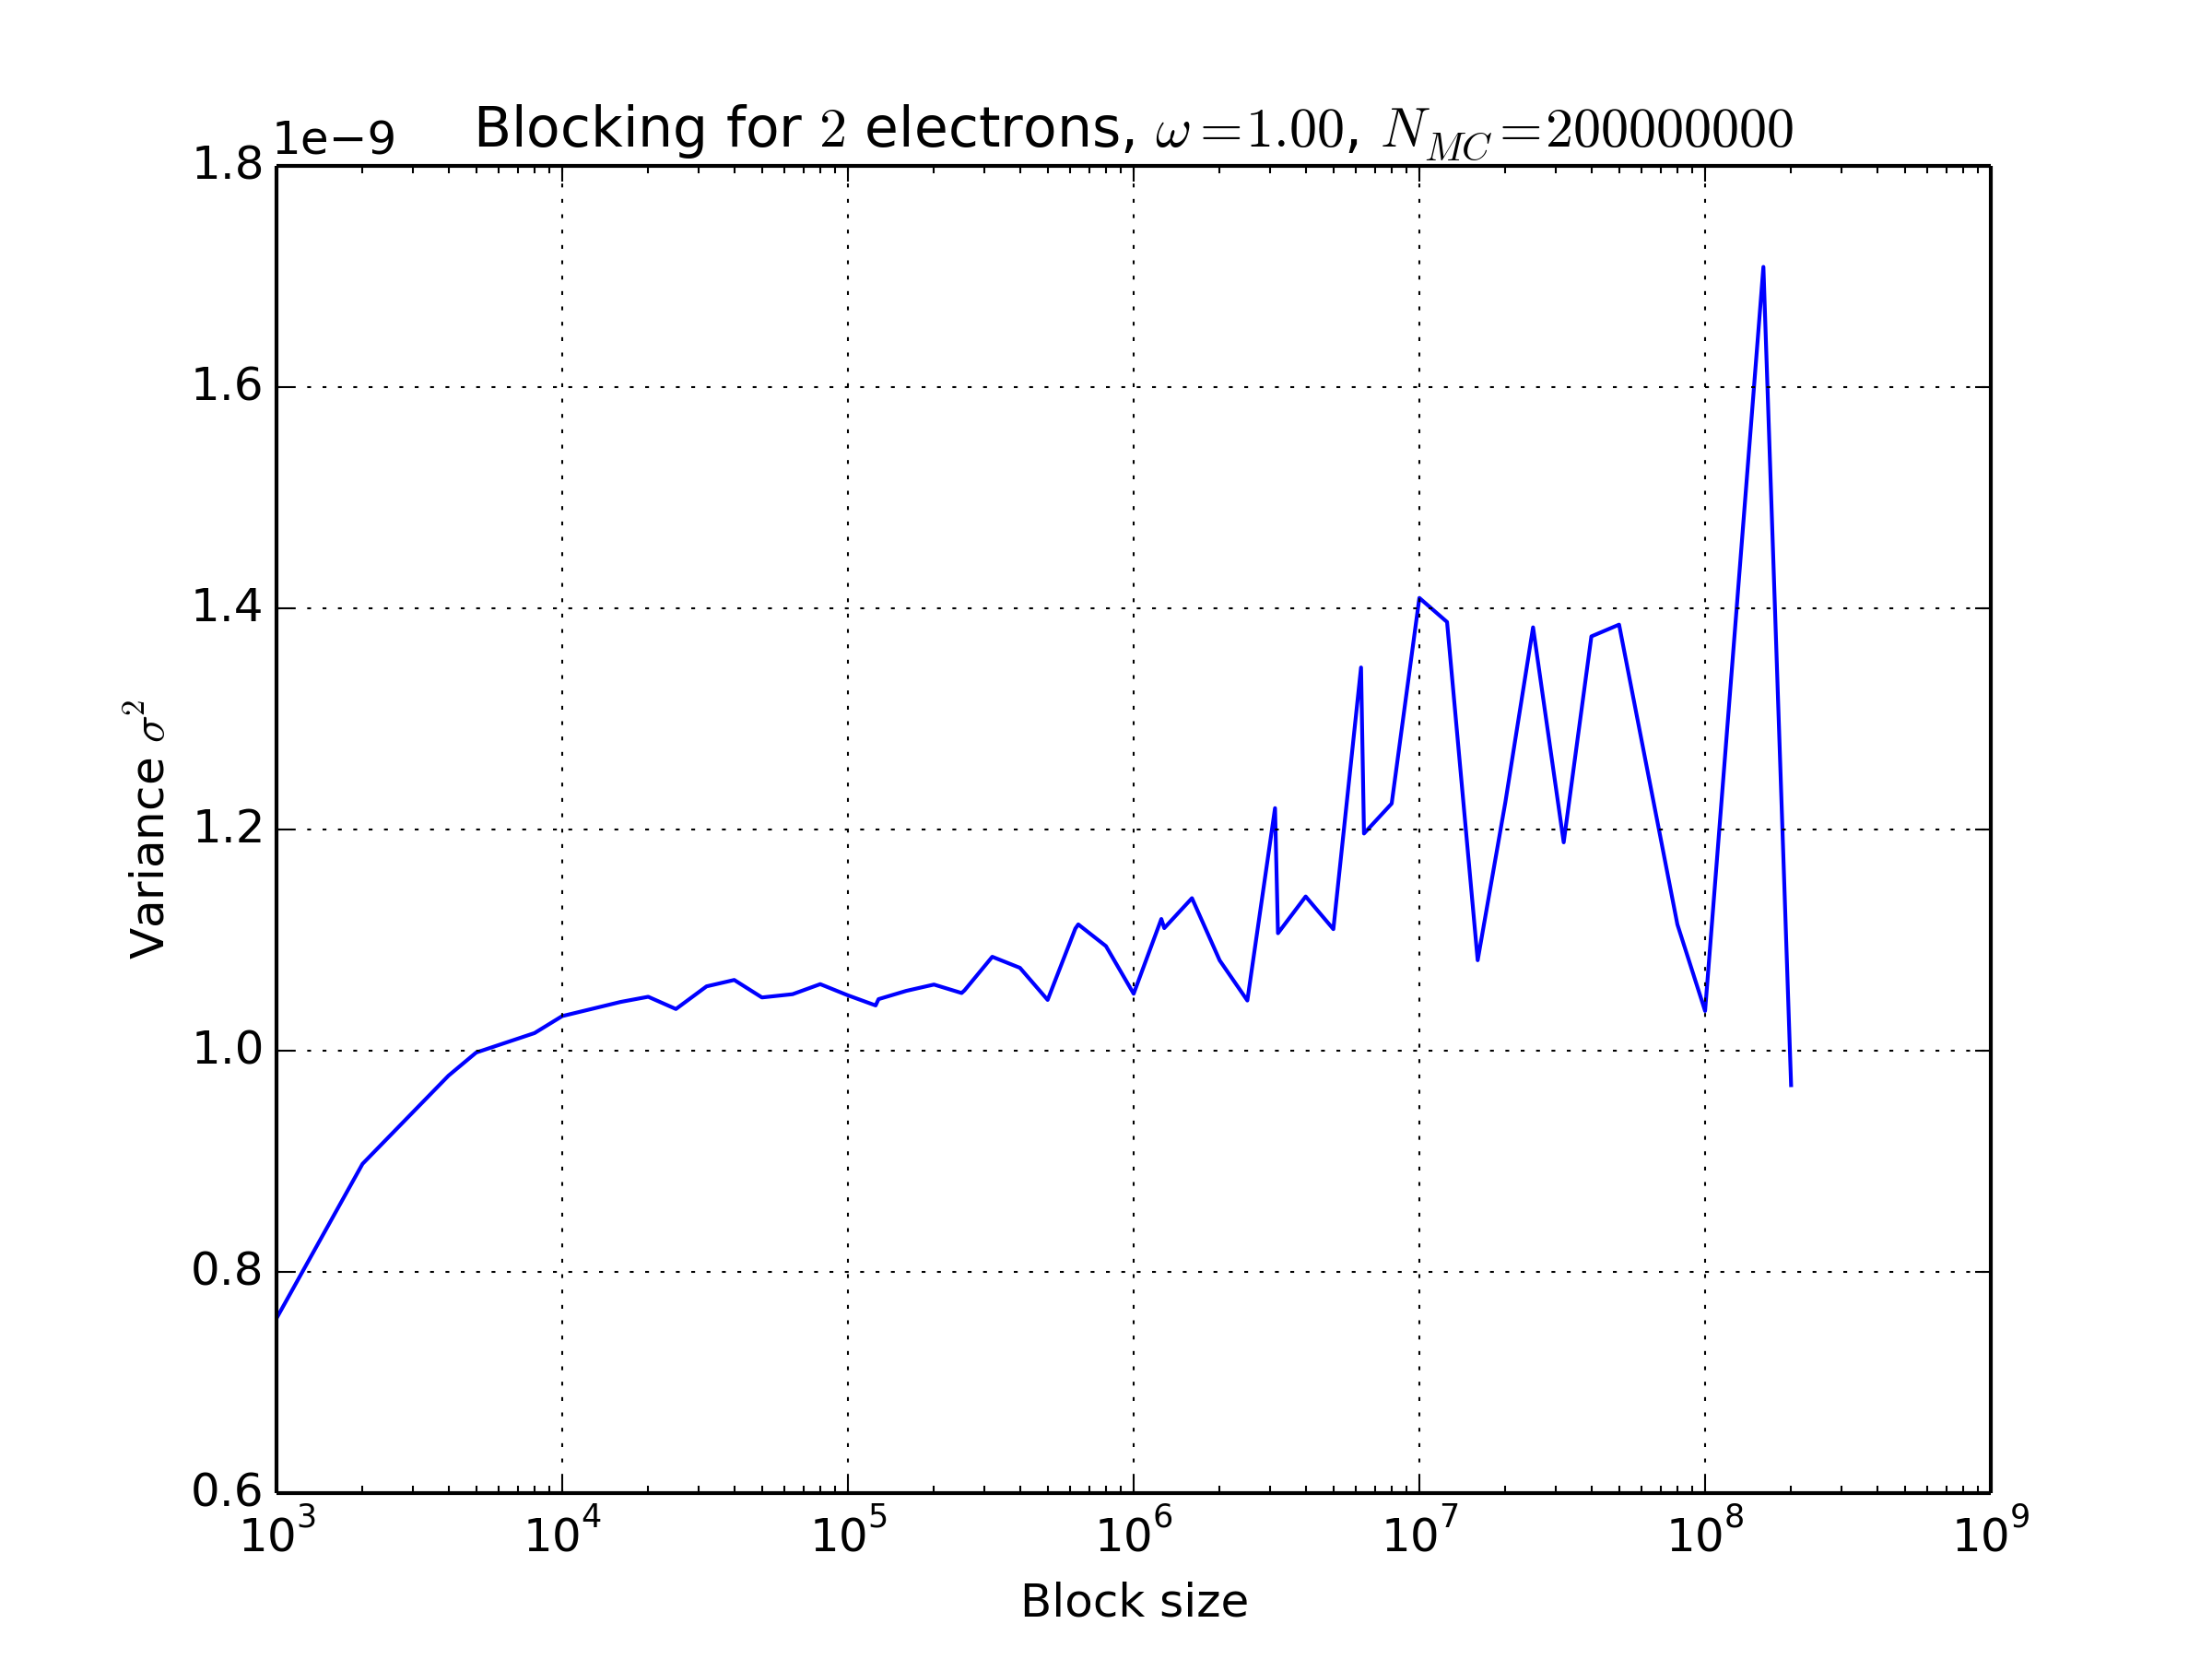
\includegraphics[width=1.0\linewidth]{../figures/figures_to_use/electron2_omega1_beta1.png} 
        \caption{With hard coded importance sampling. $2\cdot10^8$ MC samples, $\omega=1.0$.}
        \label{fig:blocking-2e-imp-hc}
    \end{subfigure}
    \hfill
    \begin{subfigure}[t]{0.45\textwidth}
        \centering
        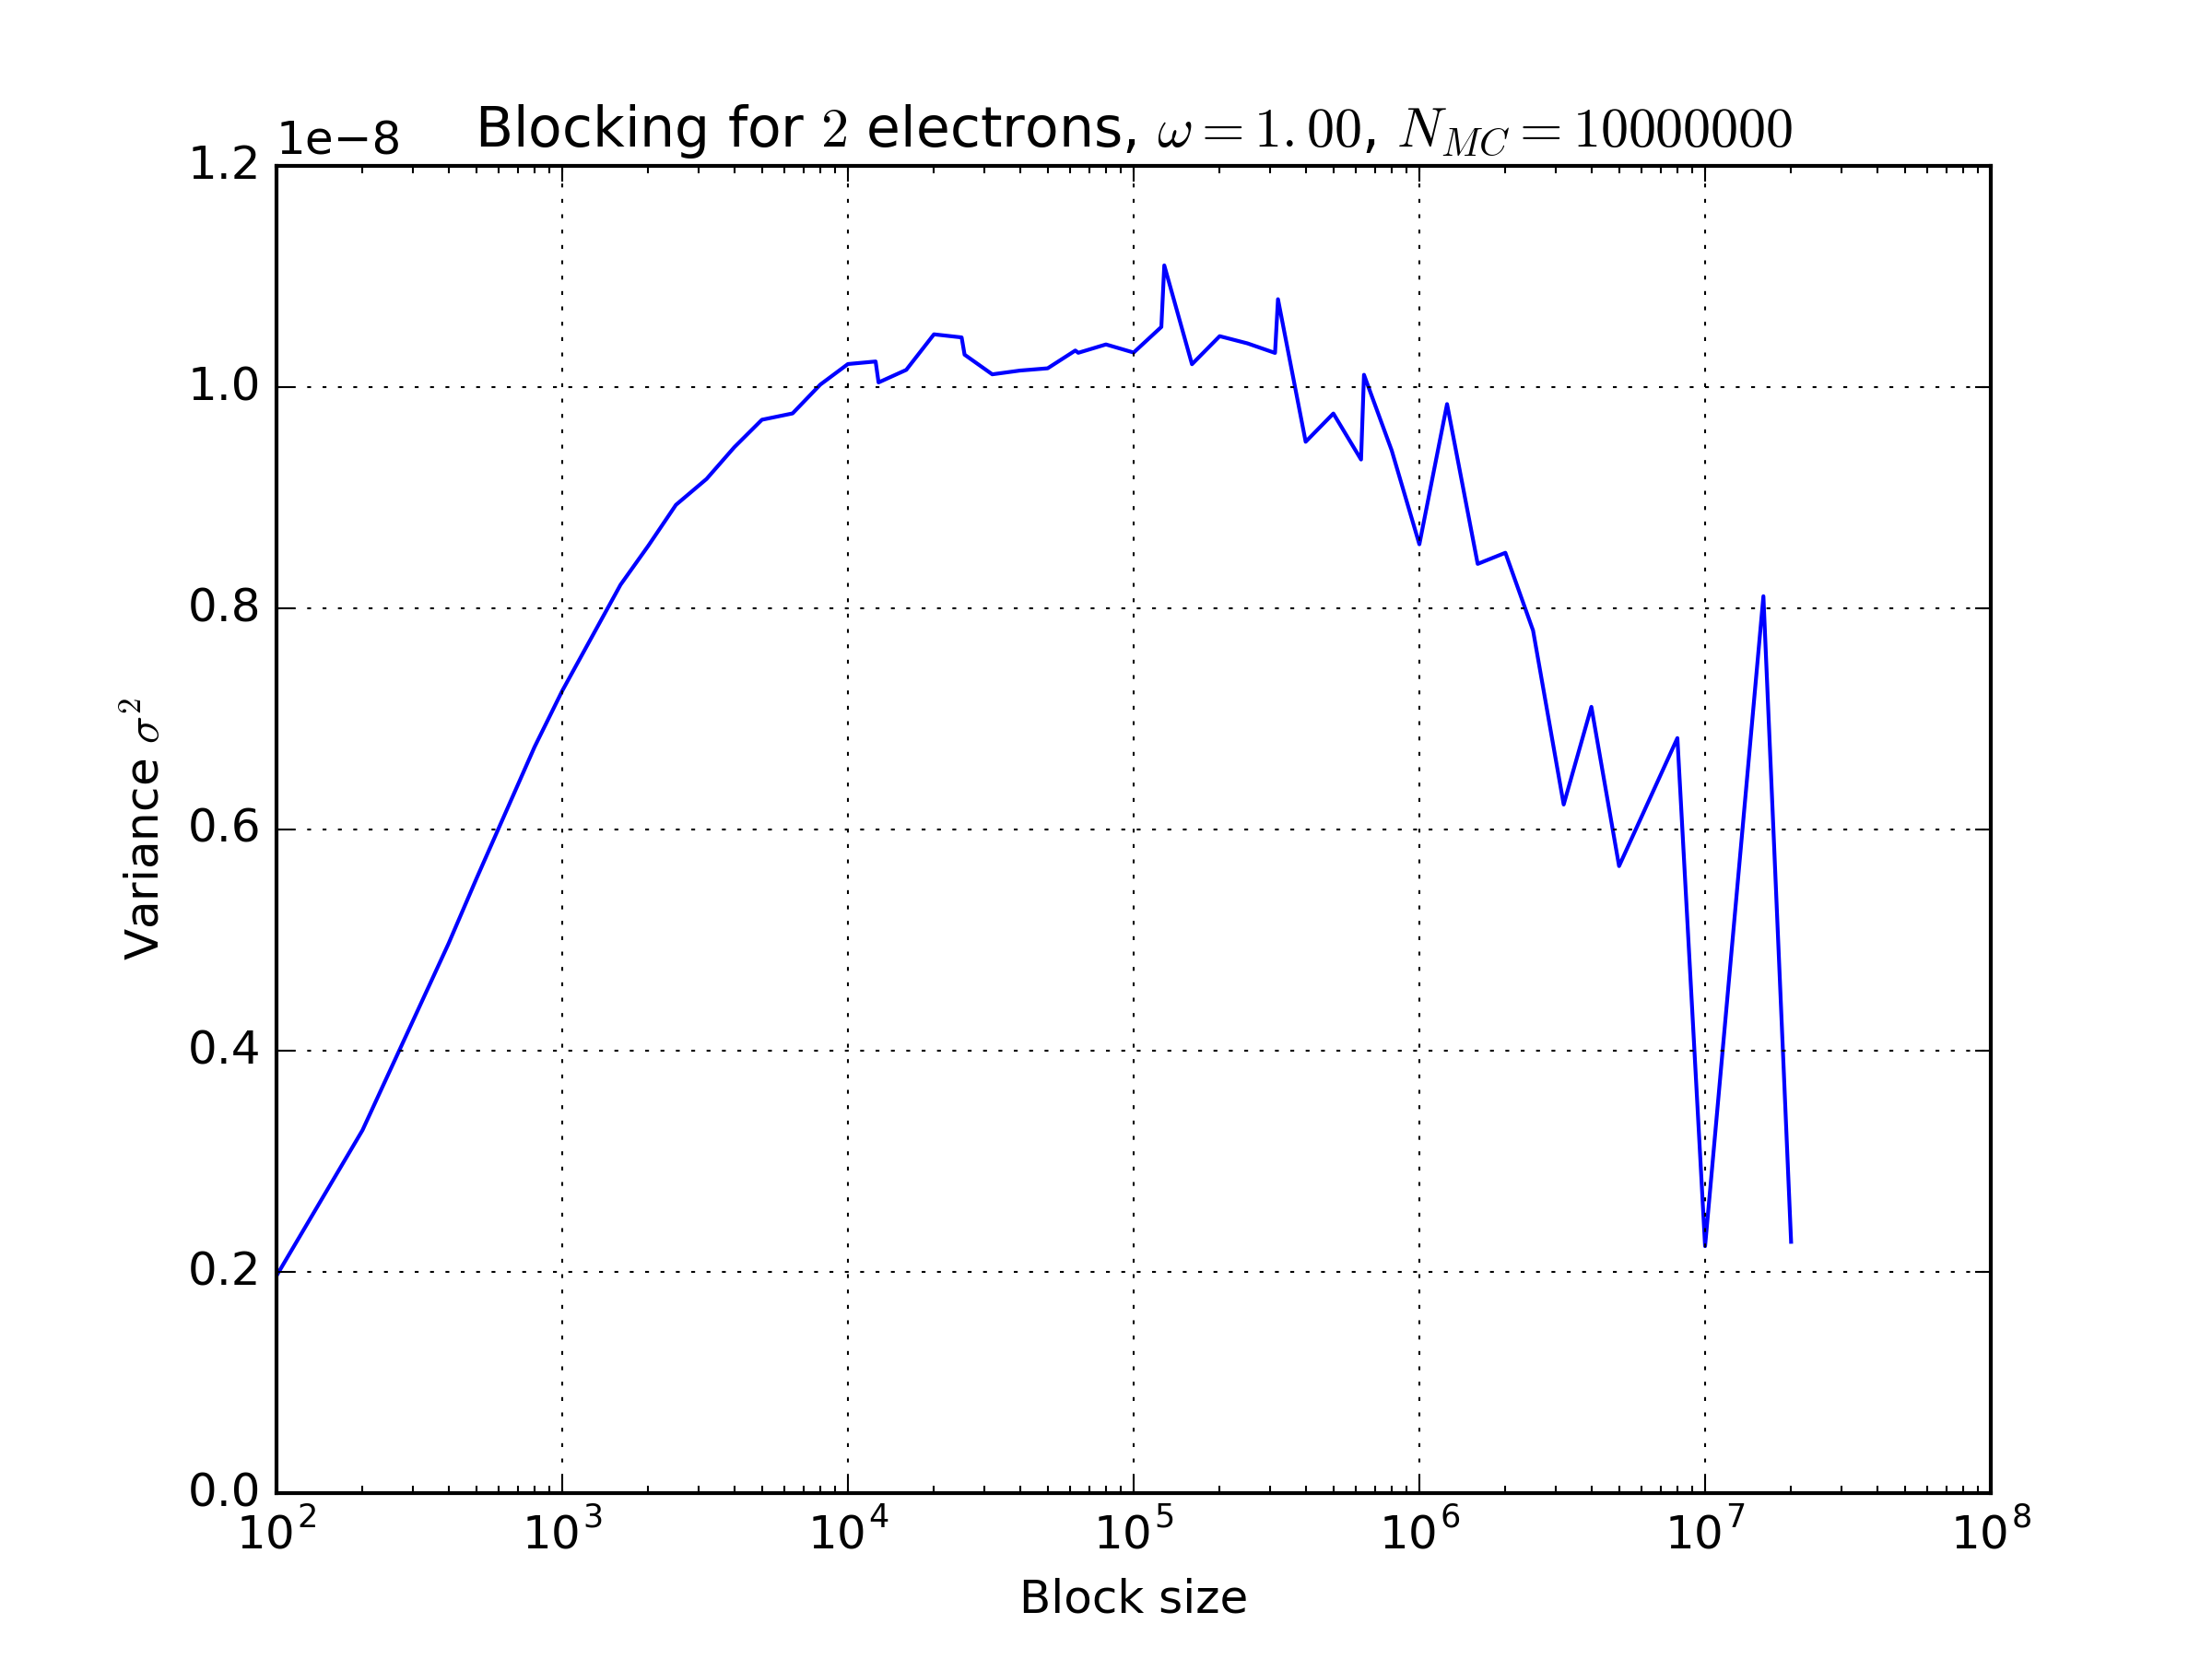
\includegraphics[width=1.0\linewidth]{../figures/figures_to_use/imp_electron2_omega1_beta1.png} 
        \caption{With importance sampling. $10^7$ MC samples, $\omega=1.0$.}
        \label{fig:blocking-2e-imp-general-method}
    \end{subfigure}
    \vspace{1cm}
    \begin{subfigure}[t]{0.45\textwidth}
        \centering
        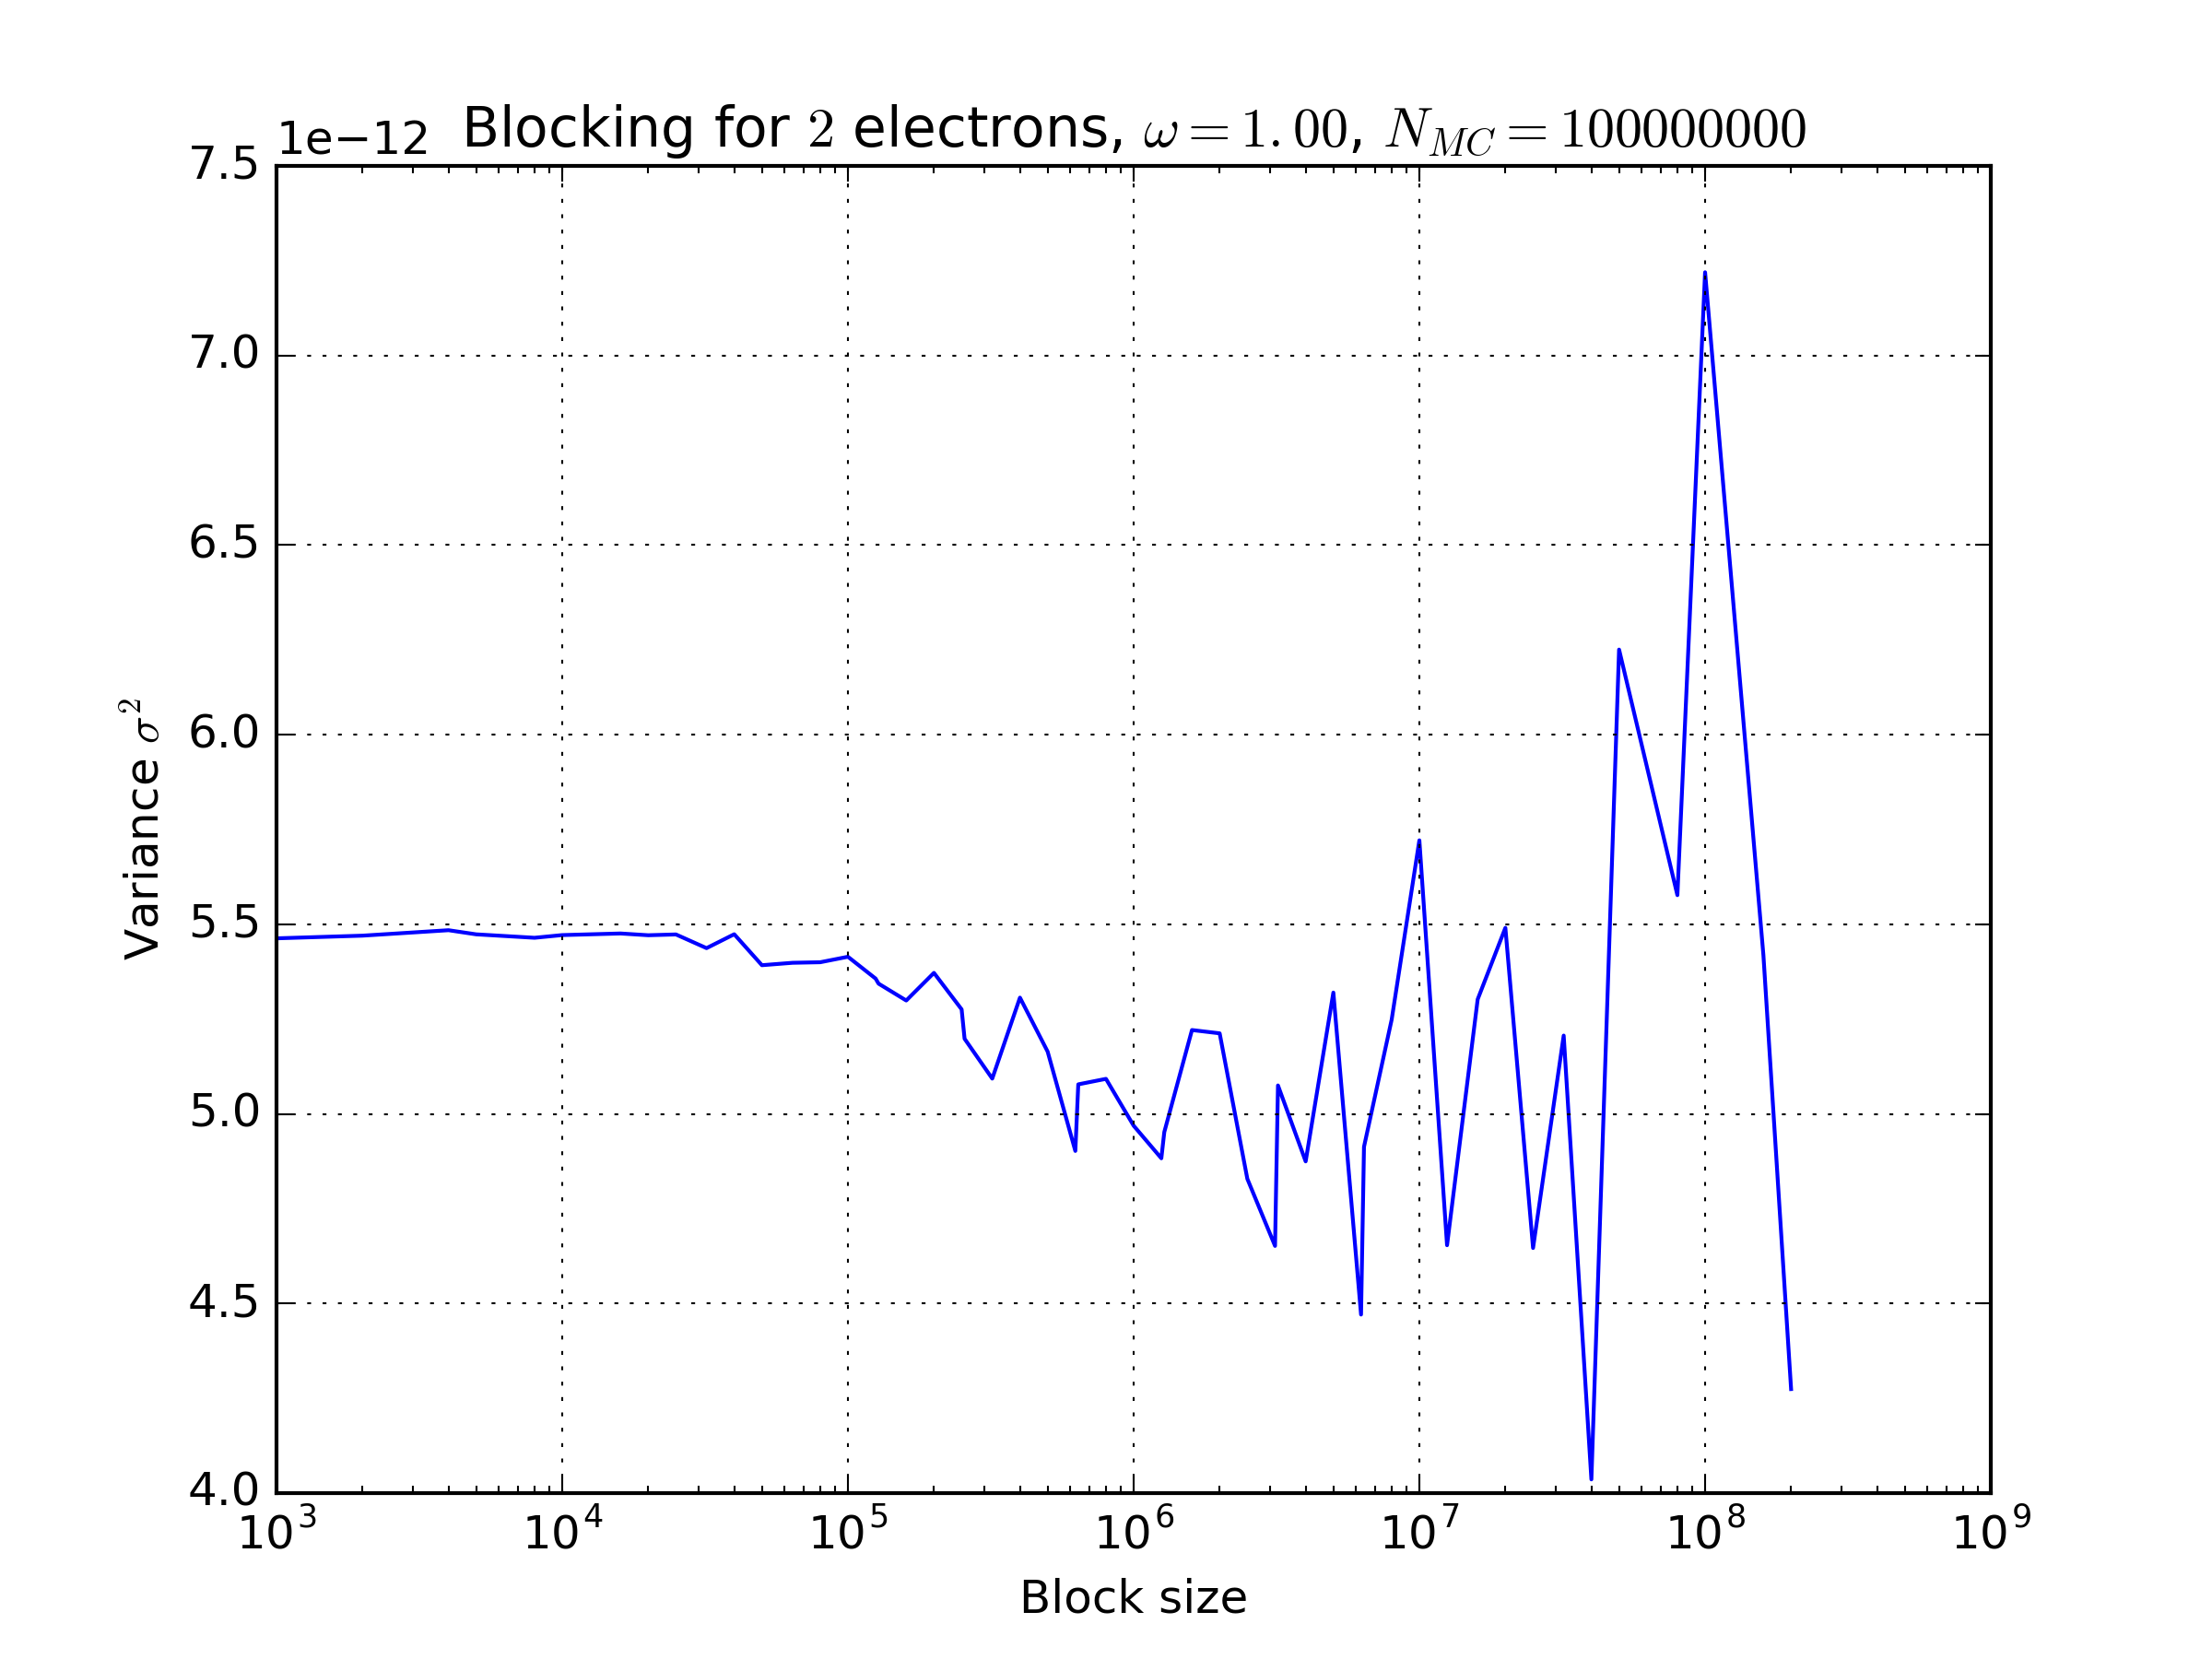
\includegraphics[width=1.0\linewidth]{../figures/figures_to_use/noImp_electron2_omega1_beta1.png} 
        \caption{2 electron case without importance sampling. $10^8$ MC samples, $\omega=1.0$.}
        \label{fig:blocking-2e-no-imp-general-method}
    \end{subfigure}
    \hfill
    \begin{subfigure}[t]{0.45\textwidth}
        \centering
        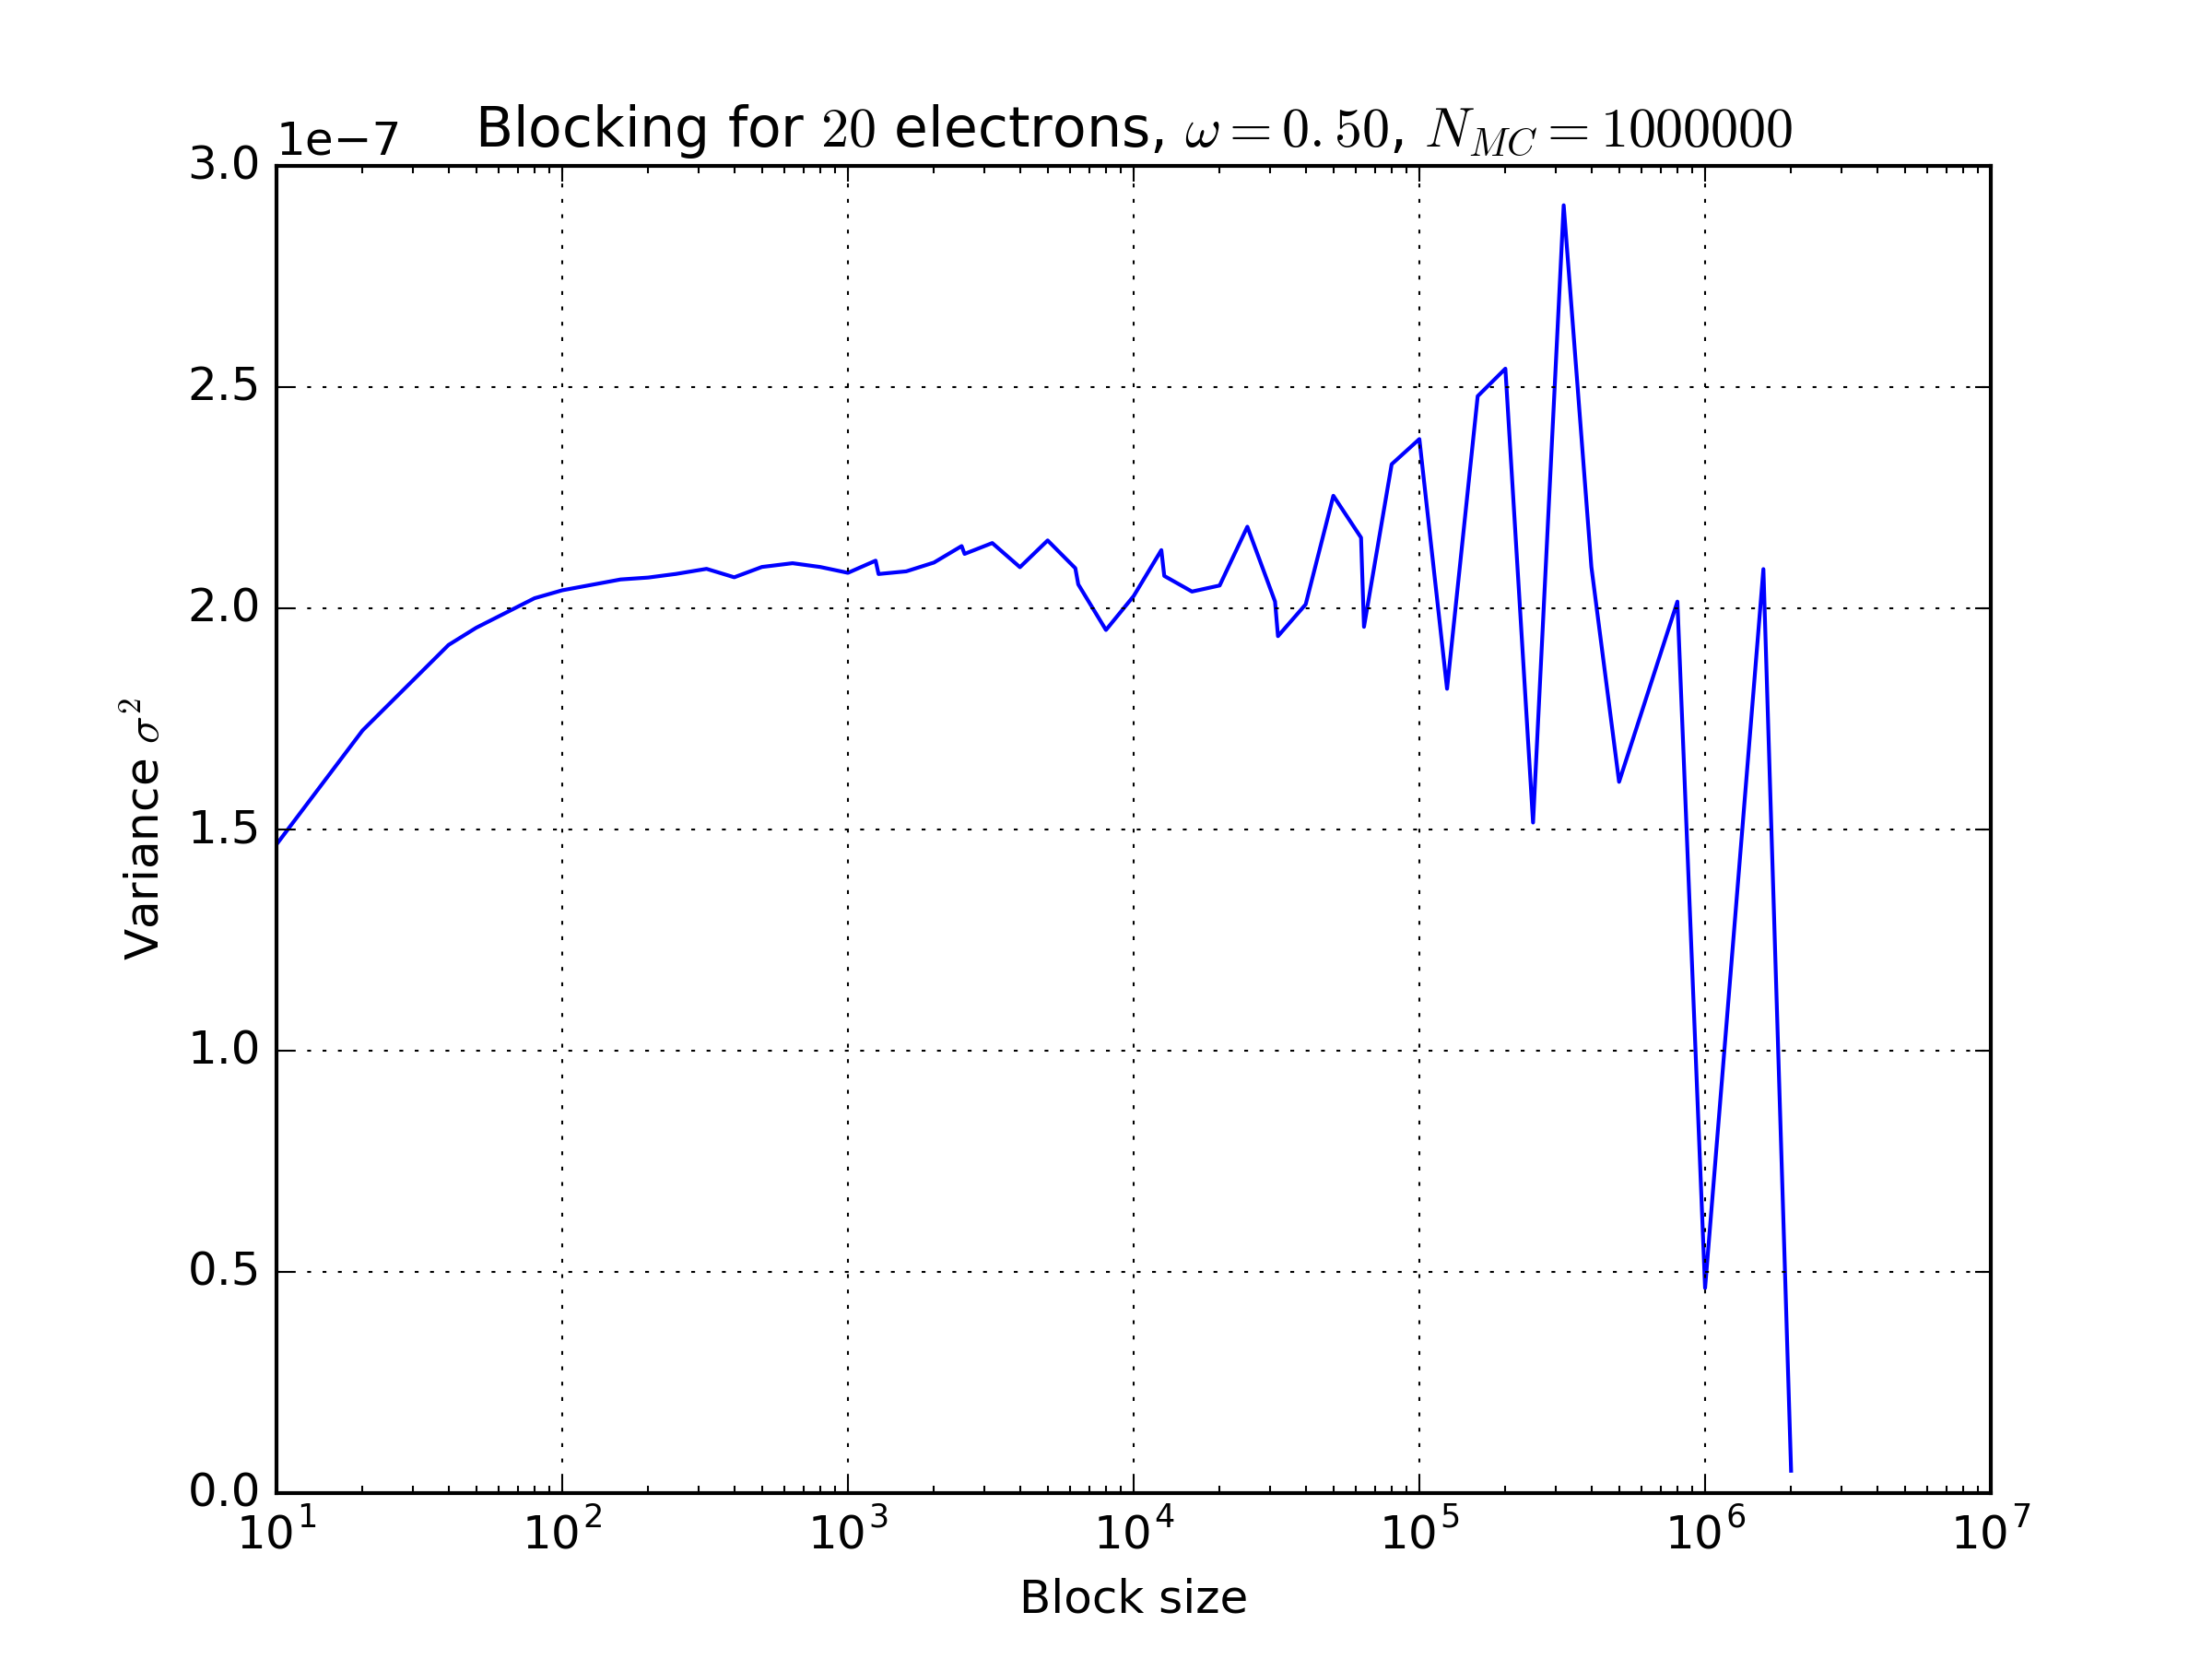
\includegraphics[width=1.0\linewidth]{../figures/figures_to_use/noImp_electron20_omega05_beta1.png} 
        \caption{20 electron case without importance sampling. $10^6$ MC samples, $\omega=0.5$.}
        \label{fig:blocking-20e-no-imp-general-method}
    \end{subfigure}
    \caption{Different plots of variance $\sigma^2$ versus different block-sizes.}
    \label{fig:blocking-plots}
\end{figure}

\subsection{Program verification and tests}
\subsubsection{Unperturbed energies}
The unperturbed energies can be viewed in the following table.

\begin{table}[H]
	\centering
	\caption{Unperturbed cases where the variational parameter $\alpha=1.0$. All results obtained using $10^6$ Monte Carlo steps and with uniform sampling.}
	\begin{tabular}{c c c c c c c c}
		\\ \hline \hline
		$N$ 			  &       $\omega$   &$\langle E \rangle$ &     $\sigma^2$ &$\langle K\rangle$ &$\langle V \rangle$ &     Accept. \\ \hline
		$              2$ &$              1$ &$              2$ &$              0$ &$        0.99887$ &$         1.0011$ & $           52.8$ \\ 
		$              2$ &$            0.5$ &$              1$ &$              0$ &$         0.4999$ &$         0.5001$ & $           51.6$ \\ 
		$              2$ &$            0.1$ &$            0.2$ &$              0$ &$       0.099835$ &$        0.10016$ & $           52.7$ \\ 
		$              2$ &$           0.05$ &$            0.1$ &$              0$ &$       0.049947$ &$       0.050053$ & $             54$ \\ 
		$              2$ &$           0.01$ &$           0.02$ &$      -10^{-20}$ &$      0.0099913$ &$       0.010009$ & $           56.1$ \\ 
		$              6$ &$              1$ &$             10$ &$              0$ &$         5.0015$ &$         4.9985$ & $           47.6$ \\ 
		$              6$ &$            0.5$ &$              5$ &$              0$ &$         2.4999$ &$         2.5001$ & $           46.5$ \\ 
		$              6$ &$            0.1$ &$              1$ &$              0$ &$        0.49971$ &$        0.50029$ & $           47.6$ \\ 
		$              6$ &$           0.05$ &$            0.5$ &$              0$ &$        0.24996$ &$        0.25004$ & $           48.8$ \\ 
		$              6$ &$           0.01$ &$            0.1$ &$              0$ &$       0.050012$ &$       0.049988$ & $           50.9$ \\ 
		$             12$ &$              1$ &$             28$ &$              0$ &$             14$ &$             14$ & $           43.8$ \\ 
		$             12$ &$            0.5$ &$             14$ &$              0$ &$         6.9998$ &$         7.0002$ & $           42.7$ \\ 
		$             12$ &$            0.1$ &$            2.8$ &$2\cdot 10^{-16}$ &$         1.3993$ &$         1.4007$ & $           43.8$ \\ 
		$             12$ &$           0.05$ &$            1.4$ &$6\cdot 10^{-17}$ &$        0.70004$ &$        0.69996$ & $           44.9$ \\ 
		$             12$ &$           0.01$ &$           0.28$ &$3\cdot 10^{-18}$ &$        0.13999$ &$        0.14001$ & $           46.9$ \\ 
		$             20$ &$              1$ &$             60$ &$              0$ &$         30.007$ &$         29.993$ & $             41$ \\ 
		$             20$ &$            0.5$ &$             30$ &$              0$ &$         14.998$ &$         15.002$ & $             40$ \\ 
		$             20$ &$            0.1$ &$              6$ &$              0$ &$         2.9986$ &$         3.0014$ & $           40.9$ \\ 
		$             20$ &$           0.05$ &$              3$ &$              0$ &$         1.4999$ &$         1.5001$ & $             42$ \\ 
		$             20$ &$           0.01$ &$            0.6$ &$-7\cdot10^{-18}$ &$        0.29996$ &$        0.30004$ & $           43.9$ \\ 
		\hline \hline
	\end{tabular}
	\label{tab:unperturbed-energies}
\end{table}

\subsubsection{\texorpdfstring{$2$}{a} electron case with and without Jastrow}
For the hard coded case with the Jastrow factor, we should get an energy that equal 3 a.u. as found by \citet{PhysRevA.48.3561} when running with Jastrow factor and Coulomb interaction. We have hard coded the two electron case without a Jastrow factor, using wave function seen in the section for the unperturbed two electron case \eqref{eq:two-body-wf} and the local energy \eqref{eq:two-electron-local-energy-unperturbed}. 

We observe that for the hard coded case with Jastrow factor and importance sampling, we have a local energy of $\langle E\rangle = 3.0004\pm 10^{-5}$ a.u.

\begin{table}[H]
	\centering
	\caption{Case (a) is for hard-coded 2 electron case with Jastrow and Coulomb included. Case (b) is for hard-coded 2 electron case with Jastrow but no Coulomb interaction. Case (c) is with neither Jastrow or Coulomb interaction included. The acceptance rate for (a) and (b) where both around $98.5\%$, while for case (c) the acceptance rate were at $56.6\%$. Energies are in atomic units.}
	\begin{tabular}{c c c c c c c c c}
		\\ \hline \hline
		Case &$\langle E \rangle$ &     $\sigma^2$ &$\langle K\rangle$ &$\langle V \rangle$ &       $\alpha$ &        $\beta$ &       $N_{MC}$ \\ \hline
		(a) &$ 3.0004$ &$        10^{-9}$ &$        0.89959$ &$         2.1008$ &$        0.99651$ &$        0.39915$ &$          2\cdot10^8$ \\ 
		(b) &$ 2.1243$ &$  2\cdot10^{-7}$ &$        0.99493$ &$         1.1294$ &$         1.0905$ &$        0.49336$ &$          2\cdot10^8$ \\ 
		(c) &$      2$ &$              0$ &$        0.54379$ &$         1.4562$ &$        0.68672$ &  -               &$          2\cdot10^8$ \\ 
		\hline \hline
	\end{tabular}
	\label{tab:hc2}
\end{table}

\subsubsection{Parallelization versus non-parallelization}
We made five runs with and without parallelization for $4\cdot 10^7$ Monte Carlo cycles on four cores.

\begin{table}[H]
	\centering
	\caption{Times for parallelization. Right column is with program run with 1 core, right one is for 4 cores. Run for 2 electrons with $\omega = 1.0$ for $N_{MC}=4\cdot10^7$.}
	\begin{tabular}{c c}
		\\ \hline \hline
		$T_1$ [s]& $T_p$ [s] \\ \hline
		22.313027 & 75.566675 \\
		22.484323 & 74.749889 \\
		22.220841 & 75.247932 \\
		22.757712 & 75.280813 \\
        \hline \hline
	\end{tabular}
	\label{tab:parallelization-times}
\end{table}

From the values listed in table \ref{tab:parallelization-times}, we get that the speed from equation \eqref{eq:parallel-speed-up} is $S(p=4) = 3.351 \pm 0.036$, and that the fraction of the program that is parallelizable is $f = 0.702 \pm 0.003$.




\section{Discussion and conclusion}
The road to achieving a satisfactory result have been long and a difficult one. The target I had in mind when starting was to create a program both flexible and efficient. While the first may be true, the latter still has a lot of potential(the author suspects another month might have been needed). 

% Introduction to problems during simulations
\subsection{Issues related to implementation}
The most pertinent issue remaining is the one regarding importance sampling for $N > 2$ electrons, in which singular matrices appear. The main suspect for this was the quantum force. After careful analysis of the code, no faults could be found and root problem remain hidden.

% uniform sampling
\subsection{Uniform sampling}
However, usable results were achievable despite implementation issues. Results using uniform sampling(see equation \eqref{tab:reg-sampling}) were presented in table \ref{tab:reg-sampling}. One worrying aspect of these results is the low variance. For cases comparable with results from importance sampling, we have almost six orders of magnitude in difference. Since the results appear to be in good agreement with cited articles, it is difficult to pinpoint exact reason for this. It should be pointed out that results without importance sampling were run with $8\cdot 10^8$ Monte Carlo cycles, while with importance sampling for only $8\cdot 10^7$ cycles. 

Instabilities for $N=12$ and $N=20$ electrons were found for small $\omega$ values. One possible remedy to this might be to decrease step size $\Delta t$, which is a possible improvement for the future.

Let us now look at three cases. For $N=6$ electrons we have $\langle E \rangle = 20.207\pm 3.0\cdot 10^{-5}$ a.u., compared to $\langle E \rangle_1 = 20.174$ a.u. For $N=12$ electrons, we have $\langle E \rangle = 65.932\pm 2.0\cdot 10^{-4}$ a.u., compared to $\langle E \rangle_1=65.741$ a.u. At last, for $N=20$ electrons, we have $\langle E \rangle = 156.31\pm 10^{-3}$ a.u. and a reference of $\langle E \rangle_1 = 155.96$ a.u. What this tells us, is that our method using \textit{uniform} sampling is correctly implemented.

% Optimal parameters from uniform sampling
\subsection{Optimal parameters from uniform sampling}
The optimal parameters found through steepest descent can be viewed in table \ref{tab:optimal-parameters}. As seen, there are no obvious outliers. No convergence criteria were implemented, nor any other methods for improving step size as one gradually creeps towards the local minimum. Had time been not been a constraint, methods for achieving an better step sizes $\Delta t$ when in the vicinity of a minimum, would have been implemented.

% Importance sampling
\subsection{Importance sampling}
Due to the error with singular matrices and thus not being able to find their inverse, importance sampling was only achievable for $N=2$ electrons. Still, we were able to produce results corresponding good with reference values as well as results obtained without importance sampling. For $\omega = 1.0$, we have results that are in close proximity for those from uniform sampling.
% \husk{Optimal parameters from importance sampling?}

% Blocking
\subsection{Blocking}
The results from blocking can be viewed in figure \ref{fig:blocking-plots}. We see that we get significant oscillations in the variance as the block-sizes increases beyond $10^6$ samples per block. As mentioned earlier, I chose block-sizes to be around $\sim 10^4-10^5$ when retrieving the optimal variances. If we look close at the plot for 2 electrons and $\omega = 1.0$ with importance sampling \ref{fig:blocking-2e-imp-general-method}, we see that from running importance sampling we get over a order of magnitude in improvement(assuming that the variance keeps increasing for continuously smaller block-sizes).

\subsection{Verification and tests}
% Unperturbed energies
A number of different tests were implemented. As we demonstrated in equation \eqref{eq:two-electron-local-energy-unperturbed}, the unperturbed energy should come out be exactly 2 a.u.(atomic unites) with zero variance for 2 electrons. For 6, 12 and 20 electrons we should get respectively $10\omega$, $28\omega$ and $60\omega$ and zero variance. From the table \ref{tab:unperturbed-energies} we observe that this is fulfilled to almost the exact decimal. By almost, I imply that we have certain instabilities for small $\omega$ values. We can also see that the acceptance ratio is not necessarily at $50\%$ either. This can be attributed to poor calibration, as one need to calibrate this to be $50\%$ for \textit{all} cases. If time were not of the essence, this could be automated. All in all, this is a good indication that our program is correct(at least for uniform sampling).
% Hardcoded electron case

From table \ref{tab:hc2} we observe three different hard-coded cases. From comparing these values with the ones obtained from the general case we have a what appears to be a good one-to-one mapping. If we look at the 2 electron case with $\omega=1.0$, for the hard coded case with importance sampling we have $\langle E\rangle=3.0004\pm10^{-5}$a.u., and for the general method we have $\langle E\rangle=3.0005\pm10^{-5}$a.u. This compared to the results obtained by \citet{PhysRevB.84.115302} $\langle E \rangle = 3.0$, we observe we have a rather good result for both hard-coded and general method. This, and the high acceptance rate($\sim 99\%$), leads us to believe that our method is working as intended.

% Parallelization
We also achieved a speedup by parallelizing our programs(the blocking method was also parallelized). For our main program, we achieved a parallelizable fraction of $f=0.702\pm 0.003$. The low $f$ is somewhat spurious, as one should expect from a naively and simple parallelization with little cross-communication to have a fraction closer to 1. Further investigation is needed to determine the cause of this.

% Final thoughts and conclusions
\subsection{Closing thoughts and remarks.}
As we now have observed, results have been obtained even though certain elements of the simulation remains out of scope. We can infer from comparing results with tests and other articles\cite{PhysRevB.84.115302}, that using uniform sampling have provided good results. Suspicion wetter the variance is correct or not still remains, but the local energy $\langle E\rangle$ appears to be within acceptable ranges. Further investigations into the root bug of using importance sampling would be interesting, but only when available time tends to infinity.

\begin{appendices}
	\section{Hermite polynomials}
	The first few Hermite polynomials in the physicists definition that will be used are given as,
	\begin{align*}
		H_0(x) = 1
	\end{align*}
	\begin{align*}
		H_1(x) = 2x
	\end{align*}
	\begin{align*}
		H_2(x) = 4x^2 - 2
	\end{align*}
	\begin{align*}
		H_3(x) = 8x^3 - 12x
	\end{align*}
	\begin{align*}
		H_4(x) = 16x^4 - 48x^2 + 12
	\end{align*}
	Their derivatives is given as
	\begin{align*}
		\frac{\partial H_0(x)}{\partial x} = 0
	\end{align*}
	\begin{align*}
		\frac{\partial H_1(x)}{\partial x} = 2
	\end{align*}
	\begin{align*}
		\frac{\partial H_2(x)}{\partial x} = 8x
	\end{align*}
	\begin{align*}
		\frac{\partial H_3(x)}{\partial x} = 24x^2 - 12
	\end{align*}
	\begin{align*}
		\frac{\partial H_4(x)}{\partial x} = 64x^3 - 96x
	\end{align*}
	Their second derivatives goes as
	\begin{align*}
		\frac{\partial^2 H_0(x)}{\partial x^2} = 0
	\end{align*}
	\begin{align*}
		\frac{\partial^2 H_1(x)}{\partial x^2} = 0
	\end{align*}
	\begin{align*}
		\frac{\partial^2 H_2(x)}{\partial x^2} = 8
	\end{align*}
	\begin{align*}
		\frac{\partial^2 H_3(x)}{\partial x^2} = 48x
	\end{align*}
	\begin{align*}
		\frac{\partial^2 H_4(x)}{\partial x^2} = 192x^2 - 96
	\end{align*}
	For finding the $\alpha$ derivative, we can use the recursive derivative relation,
	\begin{align}
		H'_n(x) = 2nH_{n-1}(x)
		\label{eq:hermite-recursive-relation}
	\end{align}

	\section{Integral formulas}
	Solution to a Gaussian integral is given as,
	\begin{align}
		\int \exp\left( - \omega x^2 \right) d x = \sqrt{\frac{\pi}{\omega}} = \sqrt{\pi}\omega^{-\frac{1}{2}}
		\label{eq:gaussian-integral}
	\end{align}
	Another symmetric Gaussian integral is given as,
	\begin{align}
		\int x^2 \exp\left( - \omega x^2 \right) d x = \frac{\sqrt{\pi}}{2}\omega^{-\frac{3}{2}}
		\label{eq:gaussian-integral-x-squared}
	\end{align}
	
	\section{Jacobi's formula}
	When finding the derivative of the Slater determinant, we will need the Jacobi formula,
	\begin{align}
		\frac{d}{dt}\det A(t) = \mathrm{tr} \left( \mathrm{adj}(A(t))\frac{dA(t)}{dt} \right)
		\label{eq:jacobi-formula}
	\end{align}
\end{appendices}

\bibliography{refs}{}
%\bibliographystyle{plain}
\bibliographystyle{plainnat}

\end{document}